\documentclass[10pt,fleqn]{article} % Default font size and left-justified equations
\usepackage[%
    pdftitle={CIN : Cinématique du solide},
    pdfauthor={Xavier Pessoles}]{hyperref}

%%%%%%%%%%%%%%%%%%%%%%%%%%%%%%%%%%%%%%%%%
% Original author:
% Mathias Legrand (legrand.mathias@gmail.com) with modifications by:
% Vel (vel@latextemplates.com)
% License:
% CC BY-NC-SA 3.0 (http://creativecommons.org/licenses/by-nc-sa/3.0/)
%%%%%%%%%%%%%%%%%%%%%%%%%%%%%%%%%%%%%%%%%

%----------------------------------------------------------------------------------------
%	VARIOUS REQUIRED PACKAGES AND CONFIGURATIONS
%----------------------------------------------------------------------------------------

\usepackage[top=2.5cm,bottom=2cm,left=2cm,right=2cm,headsep=40pt,a4paper]{geometry} % Page margins

\usepackage{graphicx} % Required for including pictures
\graphicspath{{images/}} % Specifies the directory where pictures are stored

\usepackage{lipsum} % Inserts dummy text

\usepackage{tikz} % Required for drawing custom shapes

\usepackage[french]{babel} % English language/hyphenation
\frenchbsetup{StandardLists=true} % Pour éviter la collision babel enumitem pour les listes

\usepackage{enumitem} % Customize lists
\setlist{nolistsep} % Reduce spacing between bullet points and numbered lists

\usepackage{booktabs} % Required for nicer horizontal rules in tables

\usepackage{xcolor} % Required for specifying colors by name
%\definecolor{ocre}{RGB}{243,102,25} % Define the orange color used for highlighting throughout the book
 \definecolor{ocre}{RGB}{49,133,156} % Couleur ''bleue''
\definecolor{violetf}{RGB}{112,48,160} % Couleur ''violet''
\usepackage{enumitem}
\usepackage{pifont} % Pour les dinglist
\usepackage{multicol}
\usepackage{array} % Centrage vertical dans les tableaux

%----------------------------------------------------------------------------------------
%	FONTS
%----------------------------------------------------------------------------------------

\usepackage{avant} % Use the Avantgarde font for headings
%\usepackage{times} % Use the Times font for headings
%\usepackage{mathptmx} % Use the Adobe Times Roman as the default text font together with math symbols from the Sym­bol, Chancery and Com­puter Modern fonts
\usepackage[adobe-utopia]{mathdesign}
\usepackage{microtype} % Slightly tweak font spacing for aesthetics
\usepackage[utf8]{inputenc} % Required for including letters with accents
\usepackage[T1]{fontenc} % Use 8-bit encoding that has 256 glyphs

%----------------------------------------------------------------------------------------
%	BIBLIOGRAPHY AND INDEX
%----------------------------------------------------------------------------------------

\usepackage[style=alphabetic,citestyle=numeric,sorting=nyt,sortcites=true,autopunct=true,babel=hyphen,hyperref=true,abbreviate=false,backref=true,backend=biber]{biblatex}
\addbibresource{bibliography.bib} % BibTeX bibliography file
\defbibheading{bibempty}{}

\usepackage{calc} % For simpler calculation - used for spacing the index letter headings correctly
\usepackage{makeidx} % Required to make an index
\makeindex % Tells LaTeX to create the files required for indexing

%----------------------------------------------------------------------------------------
%	MAIN TABLE OF CONTENTS
%----------------------------------------------------------------------------------------

\usepackage{titletoc} % Required for manipulating the table of contents

\setcounter{tocdepth}{2}     % Dans la table des matieres
\setcounter{secnumdepth}{2}

\contentsmargin{0cm} % Removes the default margin

% Part text styling
\titlecontents{part}[0cm]
{\addvspace{20pt}\centering\large\bfseries}
{}
{}
{}

% Chapter text styling
\titlecontents{chapter}[1.25cm] % Indentation
{\addvspace{12pt}\large\sffamily\bfseries} % Spacing and font options for chapters
{\color{ocre!60}\contentslabel[\Large\thecontentslabel]{1.25cm}\color{ocre}} % Chapter number
{\color{ocre}}  
{\color{ocre!60}\normalsize\;\titlerule*[.5pc]{.}\;\thecontentspage} % Page number

% Section text styling
\titlecontents{section}[1.25cm] % Indentation
{\addvspace{3pt}\sffamily\bfseries} % Spacing and font options for sections
{\color{ocre!60}\contentslabel[\thecontentslabel]{1.25cm} \color{ocre}} % Section number
{\color{ocre}}
{\hfill\color{ocre!60}\thecontentspage} % Page number
[]

% Subsection text styling
\titlecontents{subsection}[1.25cm] % Indentation
{\addvspace{1pt}\sffamily\small} % Spacing and font options for subsections
{\contentslabel[\thecontentslabel]{1.25cm}} % Subsection number
{}
{\ \titlerule*[.5pc]{.}\;\thecontentspage} % Page number
[]

% List of figures
\titlecontents{figure}[0em]
{\addvspace{-5pt}\sffamily}
{\thecontentslabel\hspace*{1em}}
{}
{\ \titlerule*[.5pc]{.}\;\thecontentspage}
[]

% List of tables
\titlecontents{table}[0em]
{\addvspace{-5pt}\sffamily}
{\thecontentslabel\hspace*{1em}}
{}
{\ \titlerule*[.5pc]{.}\;\thecontentspage}
[]

%----------------------------------------------------------------------------------------
%	MINI TABLE OF CONTENTS IN PART HEADS
%----------------------------------------------------------------------------------------

% Chapter text styling
\titlecontents{lchapter}[0em] % Indenting
{\addvspace{15pt}\large\sffamily\bfseries} % Spacing and font options for chapters
{\color{ocre}\contentslabel[\Large\thecontentslabel]{1.25cm}\color{ocre}} % Chapter number
{}  
{\color{ocre}\normalsize\sffamily\bfseries\;\titlerule*[.5pc]{.}\;\thecontentspage} % Page number

% Section text styling
\titlecontents{lsection}[0em] % Indenting
{\sffamily\small} % Spacing and font options for sections
{\contentslabel[\thecontentslabel]{1.25cm}} % Section number
{}
{}

% Subsection text styling
\titlecontents{lsubsection}[.5em] % Indentation
{\normalfont\footnotesize\sffamily} % Font settings
{}
{}
{}

%----------------------------------------------------------------------------------------
%	PAGE HEADERS
%----------------------------------------------------------------------------------------

\usepackage{fancyhdr} % Required for header and footer configuration



\pagestyle{fancy}
 \renewcommand{\headrulewidth}{0pt}
 \fancyhead{}
 \fancyhead[L]{%
 \noindent\begin{minipage}[c]{2.6cm}%
 
\includegraphics[width=2cm]{png/logo_lycee.png}%
 \end{minipage}}

\fancyhead[C]{\rule{8cm}{.5pt}}

 \fancyhead[R]{%
 \noindent\begin{minipage}[c]{3cm}
 \begin{flushright}
 \footnotesize{\textit{\textsf{\xxtete}}}%
 \end{flushright}
 \end{minipage}
}


\fancyfoot[C]{\rule{12cm}{.5pt}}
\renewcommand{\footrulewidth}{0.2pt}
\fancyfoot[C]{\footnotesize{\bfseries \thepage}}
\fancyfoot[L]{ 
\begin{minipage}[c]{.2\linewidth}
\noindent\footnotesize{{\xxauteur}}
\end{minipage}}


\fancyfoot[R]{\footnotesize{\xxpied}
\ifthenelse{\isodd{\value{page}}}{
\begin{tikzpicture}[overlay]
\node[shape=rectangle, 
      rounded corners = .25 cm,
	  draw= ocre,
	  line width=2pt, 
	  fill = ocre!10,
	  minimum width  = 2.5cm,
	  minimum height = 3cm,] at (\xxposongletx,\xxposonglety) {};
\node at (\xxposonglettext,\xxposonglety) {\rotatebox{90}{\textbf{\large\color{ocre}{\xxonglet}}}};
%{};
\end{tikzpicture}}{}
}
%
%
%
% Removes the header from odd empty pages at the end of chapters
\makeatletter
\renewcommand{\cleardoublepage}{
\clearpage\ifodd\c@page\else
\hbox{}
\vspace*{\fill}
\thispagestyle{empty}
\newpage
\fi}

\fancypagestyle{plain}{%
\fancyhf{} % vide l’en-tête et le pied~de~page.
%\fancyfoot[C]{\bfseries \thepage} % numéro de la page en cours en gras
% et centré en pied~de~page.
\fancyfoot[R]{\footnotesize{\xxpied}}
\fancyfoot[C]{\rule{12cm}{.5pt}}
\renewcommand{\footrulewidth}{0.2pt}
\fancyfoot[C]{\footnotesize{\bfseries \thepage}}
\fancyfoot[L]{ 
\begin{minipage}[c]{.2\linewidth}
\noindent\footnotesize{{\xxauteur}}
\end{minipage}}}



%----------------------------------------------------------------------------------------
%	THEOREM STYLES
%----------------------------------------------------------------------------------------

% Conflit avec la police adobe
%\usepackage{amsmath,amsfonts,amssymb,amsthm} % For math equations, theorems, symbols, etc
\usepackage{amsmath,amsthm}

\newcommand{\intoo}[2]{\mathopen{]}#1\,;#2\mathclose{[}}
\newcommand{\ud}{\mathop{\mathrm{{}d}}\mathopen{}}
\newcommand{\intff}[2]{\mathopen{[}#1\,;#2\mathclose{]}}
%\newtheorem{notation}{Notation}[chapter]
\newtheorem{notation}{Notation}[section]

% Boxed/framed environments
\newtheoremstyle{ocrenumbox}% % Theorem style name
{0pt}% Space above
{0pt}% Space below
{\normalfont}% % Body font
{}% Indent amount
{\small\bf\sffamily\color{ocre}}% % Theorem head font
{\;}% Punctuation after theorem head
{0.25em}% Space after theorem head
{\small\sffamily\color{ocre}\thmname{#1}\nobreakspace\thmnumber%{\@ifnotempty{#1}{}\@upn{#2}}% Theorem text (e.g. Theorem 2.1)
\thmnote{\nobreakspace\the\thm@notefont\sffamily\bfseries\color{black}---\nobreakspace#3.}} % Optional theorem note
\renewcommand{\qedsymbol}{$\blacksquare$}% Optional qed square


% Boite pour les corriges
\newtheoremstyle{correctionbox}% % Theorem style name
{0pt}% Space above
{0pt}% Space below
{\normalfont}% % Body font
{}% Indent amount
{\small\bf\sffamily\color{violet}}% % Theorem head font
{\;}% Punctuation after theorem head
{0.25em}% Space after theorem head
{\small\sffamily\color{ocre}\thmname{#1}\nobreakspace\thmnumber%{\@ifnotempty{#1}{}\@upn{#2}}% Theorem text (e.g. Theorem 2.1)
\thmnote{\nobreakspace\the\thm@notefont\sffamily\bfseries\color{black}---\nobreakspace#3.}} % Optional theorem note
\renewcommand{\qedsymbol}{$\blacksquare$}% Optional qed square



\newtheoremstyle{blacknumex}% Theorem style name
{5pt}% Space above
{5pt}% Space below
{\normalfont}% Body font
{} % Indent amount
{\small\bf\sffamily}% Theorem head font
{\;}% Punctuation after theorem head
{0.25em}% Space after theorem head
{\small\sffamily{\tiny\ensuremath{\blacksquare}}\nobreakspace\thmname{#1}\nobreakspace\thmnumber%{\@ifnotempty{#1}{}\@upn{#2}}% Theorem text (e.g. Theorem 2.1)
\thmnote{\nobreakspace\the\thm@notefont\sffamily\bfseries---\nobreakspace#3.}}% Optional theorem note

\newtheoremstyle{blacknumbox} % Theorem style name
{0pt}% Space above
{0pt}% Space below
{\normalfont}% Body font
{}% Indent amount
{\small\bf\sffamily}% Theorem head font
{\;}% Punctuation after theorem head
{0.25em}% Space after theorem head
{\small\sffamily\thmname{#1}\nobreakspace 
\thmnote{\nobreakspace\the\thm@notefont\sffamily\bfseries---\nobreakspace#3.}}% Optional theorem note

% Non-boxed/non-framed environments
\newtheoremstyle{ocrenum}% % Theorem style name
{5pt}% Space above
{5pt}% Space below
{\normalfont}% % Body font
{}% Indent amount
{\small\bf\sffamily\color{ocre}}% % Theorem head font
{\;}% Punctuation after theorem head
{0.25em}% Space after theorem head
{\small\sffamily\color{ocre}\thmname{#1}\nobreakspace\thmnumber{\@ifnotempty{#1}{}\@upn{#2}}% Theorem text (e.g. Theorem 2.1)
\thmnote{\nobreakspace\the\thm@notefont\sffamily\bfseries\color{black}---\nobreakspace#3.}} % Optional theorem note
\renewcommand{\qedsymbol}{$\blacksquare$}% Optional qed square
\makeatother

% Environnement pour les titres de parties
\newtheoremstyle{partiebox} 
{0pt}% Space above
{0pt}% Space below
{\normalfont}% Body font
{}% Indent amount
{\small\bf\sffamily}% Theorem head font
{\;}% Punctuation after theorem head
{0.25em}% Space after theorem head




% Defines the theorem text style for each type of theorem to one of the three styles above
\newcounter{dummy} 
\numberwithin{dummy}{section}
\theoremstyle{ocrenumbox}
%\newtheorem{theoremeT}[dummy]{Théorème}
\newtheorem{theoremeT}[dummy]{Théorème}
\newtheorem{resultatT}[dummy]{Résultat}
\newtheorem{savoirT}[dummy]{Savoir}
\newtheorem{methodeT}[dummy]{Méthode}
\newtheorem{objectifT}[dummy]{Objectif}
%\newtheorem{problem}{Problem}[chapter]
\newtheorem{problem}{Problem}[section]
%\newtheorem{exerciseT}{Exercise}[chapter]
\newtheorem{exerciseT}{Exercice}[section]

\theoremstyle{blacknumex}
%\newtheorem{exampleT}{Example}[chapter]
\newtheorem{exempleT}{Exemple}[section]
\newtheorem{termT}{Terminal\\}[section]
\newtheorem{pyT}{Python\\}[section]
\newtheorem{sciT}{Scilab\\}[section]

\theoremstyle{blacknumbox}
%\newtheorem{vocabulary}{Vocabulary}[chapter]
\newtheorem{vocabulary}{Vocabulaire}[section]
%\newtheorem{definitionT}{Definition}[section]
\newtheorem{definitionT}{Définition}[section]
\newtheorem{demoT}{Démonstration}[section]
\newtheorem{corollaryT}[dummy]{Corollaire}
\newtheorem{hypoT}{Hypothèse(s)}

\theoremstyle{ocrenum}
\newtheorem{proposition}[dummy]{Proposition}

\theoremstyle{partiebox}
\newtheorem{titrepartieT}[]{}
\newtheorem{titrechapitreT}[]{}

\theoremstyle{correctionbox}
\newtheorem{correctionT}[dummy]{\color{violet}{Correction}}

%----------------------------------------------------------------------------------------
%	DEFINITION OF COLORED BOXES
%----------------------------------------------------------------------------------------

\RequirePackage[framemethod=tikz]{mdframed} % Required for creating the theorem, definition, exercise and corollary boxes

% Theorem box
\newmdenv[skipabove=7pt,
skipbelow=7pt,
backgroundcolor=ocre!10,
linecolor=ocre,
innerleftmargin=5pt,
innerrightmargin=5pt,
innertopmargin=5pt,
leftmargin=0cm,
rightmargin=0cm,
innerbottommargin=5pt]{tBox}


% Correction
\newmdenv[skipabove=7pt,
skipbelow=7pt,
backgroundcolor=violet!10,
linecolor=violet,
innerleftmargin=5pt,
innerrightmargin=5pt,
innertopmargin=5pt,
leftmargin=0cm,
rightmargin=0cm,
innerbottommargin=5pt]{coBox}


% Exercise box	  
\newmdenv[skipabove=7pt,
skipbelow=7pt,
rightline=false,
leftline=true,
topline=false,
bottomline=false,
backgroundcolor=ocre!10,
linecolor=ocre,
innerleftmargin=5pt,
innerrightmargin=5pt,
innertopmargin=5pt,
innerbottommargin=5pt,
leftmargin=0cm,
rightmargin=0cm,
linewidth=4pt]{eBox}	

% Definition box
\newmdenv[skipabove=7pt,
skipbelow=7pt,
rightline=false,
leftline=true,
topline=false,
bottomline=false,
backgroundcolor=ocre!10,
linecolor=ocre,
innerleftmargin=5pt,
innerrightmargin=5pt,
innertopmargin=0pt,
leftmargin=0cm,
rightmargin=0cm,
linewidth=4pt,
innerbottommargin=0pt]{dBox}	

% Demonstration box
\newmdenv[skipabove=7pt,
skipbelow=7pt,
rightline=false,
leftline=true,
topline=false,
bottomline=false,
%backgroundcolor=ocre!10,
linecolor=ocre,
innerleftmargin=5pt,
innerrightmargin=5pt,
innertopmargin=0pt,
leftmargin=0cm,
rightmargin=0cm,
linewidth=4pt,
innerbottommargin=0pt]{demoBox}	

% Corollary box
\newmdenv[skipabove=7pt,
skipbelow=7pt,
rightline=false,
leftline=true,
topline=false,
bottomline=false,
linecolor=gray,
backgroundcolor=black!5,
innerleftmargin=5pt,
innerrightmargin=5pt,
innertopmargin=5pt,
leftmargin=0cm,
rightmargin=0cm,
linewidth=4pt,
innerbottommargin=5pt]{cBox}


% Hypothèses
\newmdenv[skipabove=7pt,
skipbelow=7pt,
rightline=false,
leftline=true,
topline=false,
bottomline=false,
linecolor=gray,
backgroundcolor=black!5,
innerleftmargin=5pt,
innerrightmargin=5pt,
innertopmargin=5pt,
leftmargin=0cm,
rightmargin=0cm,
linewidth=4pt,
innerbottommargin=5pt]{hyBox}


% Boite pour le titre de la partie (pBox)
\newmdenv[skipabove=7pt,
skipbelow=7pt,
rightline=true,
leftline=false,
topline=false,
bottomline=false,
linecolor=ocre,
backgroundcolor=none,
innerleftmargin=5pt,
innerrightmargin=5pt,
innertopmargin=5pt,
leftmargin=0cm,
rightmargin=0cm,
linewidth=4pt,
innerbottommargin=5pt]{pBox}

% Boite pour le titre du chapitre (chBox)
\newmdenv[skipabove=7pt,
skipbelow=7pt,
rightline=false,
leftline=true,
topline=false,
bottomline=false,
linecolor=ocre,
%backgroundcolor=black!5,
innerleftmargin=5pt,
innerrightmargin=5pt,
innertopmargin=5pt,
leftmargin=0cm,
rightmargin=0cm,
linewidth=4pt,
innerbottommargin=5pt]{chBox}


% Boite pour les exemples
\newmdenv[skipabove=7pt,
skipbelow=7pt,
rightline=false,
leftline=true,
topline=false,
bottomline=false,
linecolor=gray,
backgroundcolor=white,
innerleftmargin=5pt,
innerrightmargin=5pt,
innertopmargin=5pt,
leftmargin=0cm,
rightmargin=0cm,
linewidth=4pt,
innerbottommargin=5pt]{exBox}

% Boite pour le terminal
\newmdenv[skipabove=7pt,
skipbelow=7pt,
rightline=false,
leftline=true,
topline=false,
bottomline=false,
linecolor=gray,
backgroundcolor=white,
innerleftmargin=5pt,
innerrightmargin=5pt,
innertopmargin=5pt,
leftmargin=0cm,
rightmargin=0cm,
linewidth=4pt,
innerbottommargin=5pt]{termBox}


% Boite pour Python
\newmdenv[skipabove=7pt,
skipbelow=7pt,
rightline=false,
leftline=true,
topline=false,
bottomline=false,
linecolor=gray,
backgroundcolor=white,
innerleftmargin=5pt,
innerrightmargin=5pt,
innertopmargin=5pt,
leftmargin=0cm,
rightmargin=0cm,
linewidth=4pt,
innerbottommargin=5pt]{pyBox}

% Boite pour scilab
\newmdenv[skipabove=7pt,
skipbelow=7pt,
rightline=false,
leftline=true,
topline=false,
bottomline=false,
linecolor=gray,
backgroundcolor=white,
innerleftmargin=5pt,
innerrightmargin=5pt,
innertopmargin=5pt,
leftmargin=0cm,
rightmargin=0cm,
linewidth=4pt,
innerbottommargin=5pt]{sciBox}
% Creates an environment for each type of theorem and assigns it a theorem text style from the "Theorem Styles" section above and a colored box from above
\newenvironment{theorem}{\begin{tBox}\begin{theoremeT}}{\end{theoremeT}\end{tBox}}
\newenvironment{resultat}{\begin{tBox}\begin{resultatT}}{\end{resultatT}\end{tBox}}
\newenvironment{methode}{\begin{tBox}\begin{methodeT}}{\end{methodeT}\end{tBox}}
\newenvironment{savoir}{\begin{tBox}\begin{savoirT}}{\end{savoirT}\end{tBox}}
\newenvironment{obj}{\begin{tBox}\begin{objectifT}}{\end{objectifT}\end{tBox}}
\newenvironment{corrige}{\begin{coBox}\begin{correctionT}}{\end{correctionT}\end{coBox}}
\newenvironment{exercise}{\begin{eBox}\begin{exerciseT}}{\hfill{\color{ocre}\tiny\ensuremath{\blacksquare}}\end{exerciseT}\end{eBox}}				  
\newenvironment{exercice}{\begin{eBox}\begin{exerciseT}}{\hfill{\color{ocre}\tiny\ensuremath{\blacksquare}}\end{exerciseT}\end{eBox}}				  

\newenvironment{definition}{\begin{dBox}\begin{definitionT}}{\end{definitionT}\end{dBox}}	
\newenvironment{defi}{\begin{dBox}\begin{definitionT}}{\end{definitionT}\end{dBox}}	
\newenvironment{demo}{\begin{demoBox}\begin{demoT}}{\end{demoT}\end{demoBox}}	
%\newenvironment{exemple}{\begin{exempleT}}{\hfill{\tiny\ensuremath{\blacksquare}}\end{exempleT}}		
\newenvironment{corollary}{\begin{cBox}\begin{corollaryT}}{\end{corollaryT}\end{cBox}}
\newenvironment{hypo}{\begin{hyBox}\begin{hypoT}}{\end{hypoT}\end{hyBox}}	\newenvironment{exemple}{\begin{exBox}\begin{exempleT}}{\hfill{\tiny\ensuremath{\blacksquare}}\end{exempleT}\end{exBox}}	
\newenvironment{titrepartie}{\begin{pBox}\begin{titrepartieT}}{\end{titrepartieT}\end{pBox}}	
\newenvironment{titrechapitre}{\begin{chBox}\begin{titrechapitreT}}{\end{titrechapitreT}\end{chBox}}	

\newenvironment{term}{ \begin{termBox}\begin{termT}}{\end{termT}\end{termBox}}
\newenvironment{py}{ \begin{pyBox}\begin{pyT}}{\end{pyT}\end{pyBox}}
\newenvironment{sci}{ \begin{sciBox}\begin{sciT}}{\end{sciT}\end{sciBox}}

%----------------------------------------------------------------------------------------
%	REMARK ENVIRONMENT
%----------------------------------------------------------------------------------------

\newenvironment{remark}{\par\vspace{10pt}\small % Vertical white space above the remark and smaller font size
\begin{list}{}{
\leftmargin=35pt % Indentation on the left
\rightmargin=25pt}\item\ignorespaces % Indentation on the right
\makebox[-2.5pt]{\begin{tikzpicture}[overlay]
\node[draw=ocre!60,line width=1pt,circle,fill=ocre!25,font=\sffamily\bfseries,inner sep=2pt,outer sep=0pt] at (-15pt,0pt){\textcolor{ocre}{R}};\end{tikzpicture}} % Orange R in a circle
\advance\baselineskip -1pt}{\end{list}\vskip5pt} % Tighter line spacing and white space after remark

\newenvironment{rem}{\par\vspace{10pt}\small % Vertical white space above the remark and smaller font size
\begin{list}{}{
\leftmargin=35pt % Indentation on the left
\rightmargin=25pt}\item\ignorespaces % Indentation on the right
\makebox[-2.5pt]{\begin{tikzpicture}[overlay]
\node[draw=ocre!60,line width=1pt,circle,fill=ocre!25,font=\sffamily\bfseries,inner sep=2pt,outer sep=0pt] at (-15pt,0pt){\textcolor{ocre}{R}};\end{tikzpicture}} % Orange R in a circle
\advance\baselineskip -1pt}{\end{list}\vskip5pt} % Tighter line spacing and white space after remark


\newenvironment{warn}{\par\vspace{10pt}\small % Vertical white space above the remark and smaller font size
\begin{list}{}{
\leftmargin=35pt % Indentation on the left
\rightmargin=25pt}\item\ignorespaces % Indentation on the right
\makebox[-2.5pt]{\begin{tikzpicture}[overlay]
\node[draw=red!60,line width=1pt,circle,fill=red!25,font=\sffamily\bfseries,inner sep=2pt,outer sep=0pt] at (-15pt,0pt){\textcolor{black}{!}};\end{tikzpicture}} % Point d'exclamation dans un cercle
\advance\baselineskip -1pt}{\end{list}\vskip5pt} % Tighter line spacing and white space after remark


%----------------------------------------------------------------------------------------
%	SECTION NUMBERING IN THE MARGIN
%----------------------------------------------------------------------------------------

\makeatletter
\renewcommand{\@seccntformat}[1]{\llap{\textcolor{ocre}{\csname the#1\endcsname}\hspace{1em}}}                    
\renewcommand{\section}{\@startsection{section}{1}{\z@}
{-4ex \@plus -1ex \@minus -.4ex}
{1ex \@plus.2ex }
{\normalfont\large\sffamily\bfseries}}
\renewcommand{\subsection}{\@startsection {subsection}{2}{\z@}
{-3ex \@plus -0.1ex \@minus -.4ex}
{0.5ex \@plus.2ex }
{\normalfont\sffamily\bfseries}}
\renewcommand{\subsubsection}{\@startsection {subsubsection}{3}{\z@}
{-2ex \@plus -0.1ex \@minus -.2ex}
{.2ex \@plus.2ex }
{\normalfont\small\sffamily\bfseries}}                        
\renewcommand\paragraph{\@startsection{paragraph}{4}{\z@}
{-2ex \@plus-.2ex \@minus .2ex}
{.1ex}
{\normalfont\small\sffamily\bfseries}}

%----------------------------------------------------------------------------------------
%	PART HEADINGS
%----------------------------------------------------------------------------------------


%----------------------------------------------------------------------------------------
%	CHAPTER HEADINGS
%----------------------------------------------------------------------------------------

% \newcommand{\thechapterimage}{}%
% \newcommand{\chapterimage}[1]{\renewcommand{\thechapterimage}{#1}}%
% \def\@makechapterhead#1{%
% {\parindent \z@ \raggedright \normalfont
% \ifnum \c@secnumdepth >\m@ne
% \if@mainmatter
% \begin{tikzpicture}[remember picture,overlay]
% \node at (current page.north west)
% {\begin{tikzpicture}[remember picture,overlay]
% \node[anchor=north west,inner sep=0pt] at (0,0) {\includegraphics[width=\paperwidth]{\thechapterimage}};
% \draw[anchor=west] (\Gm@lmargin,-9cm) node [line width=2pt,rounded corners=15pt,draw=ocre,fill=white,fill opacity=0.5,inner sep=15pt]{\strut\makebox[22cm]{}};
% \draw[anchor=west] (\Gm@lmargin+.3cm,-9cm) node {\huge\sffamily\bfseries\color{black}\thechapter. #1\strut};
% \end{tikzpicture}};
% \end{tikzpicture}
% \else
% \begin{tikzpicture}[remember picture,overlay]
% \node at (current page.north west)
% {\begin{tikzpicture}[remember picture,overlay]
% \node[anchor=north west,inner sep=0pt] at (0,0) {\includegraphics[width=\paperwidth]{\thechapterimage}};
% \draw[anchor=west] (\Gm@lmargin,-9cm) node [line width=2pt,rounded corners=15pt,draw=ocre,fill=white,fill opacity=0.5,inner sep=15pt]{\strut\makebox[22cm]{}};
% \draw[anchor=west] (\Gm@lmargin+.3cm,-9cm) node {\huge\sffamily\bfseries\color{black}#1\strut};
% \end{tikzpicture}};
% \end{tikzpicture}
% \fi\fi\par\vspace*{270\p@}}}

%-------------------------------------------

\def\@makeschapterhead#1{%
\begin{tikzpicture}[remember picture,overlay]
\node at (current page.north west)
{\begin{tikzpicture}[remember picture,overlay]
\node[anchor=north west,inner sep=0pt] at (0,0) {\includegraphics[width=\paperwidth]{\thechapterimage}};
\draw[anchor=west] (\Gm@lmargin,-9cm) node [line width=2pt,rounded corners=15pt,draw=ocre,fill=white,fill opacity=0.5,inner sep=15pt]{\strut\makebox[22cm]{}};
\draw[anchor=west] (\Gm@lmargin+.3cm,-9cm) node {\huge\sffamily\bfseries\color{black}#1\strut};
\end{tikzpicture}};
\end{tikzpicture}
\par\vspace*{270\p@}}
\makeatother

%----------------------------------------------------------------------------------------
%	HYPERLINKS IN THE DOCUMENTS
%----------------------------------------------------------------------------------------


\hypersetup{hidelinks,backref=true,pagebackref=true,hyperindex=true,colorlinks=false,breaklinks=true,urlcolor= ocre,bookmarks=true,bookmarksopen=false,pdftitle={Title},pdfauthor={Author}}
\usepackage{bookmark}
\bookmarksetup{
open,
numbered,
addtohook={%
\ifnum\bookmarkget{level}=0 % chapter
\bookmarksetup{bold}%
\fi
\ifnum\bookmarkget{level}=-1 % part
\bookmarksetup{color=ocre,bold}%
\fi
}
}

%----------------------------------------------------------------------------------------
%	
%----------------------------------------------------------------------------------------

\newcommand{\thechapterimage}{}%
\newcommand{\chapterimage}[1]{\renewcommand{\thechapterimage}{#1}}%
\def\@makechapterhead#1{%
{\parindent \z@ \raggedright \normalfont
\begin{tikzpicture}[remember picture,overlay]
\node at (current page.north west)
{\begin{tikzpicture}[remember picture,overlay]
\node[anchor=north west,inner sep=0pt] at (0,0) {\includegraphics[width=\paperwidth]{\thechapterimage}};
%\draw[anchor=west] (\Gm@lmargin,-9cm) node [line width=2pt,rounded corners=15pt,draw=ocre,fill=white,fill opacity=0.5,inner sep=15pt]{\strut\makebox[22cm]{}};
%\draw[anchor=west] (\Gm@lmargin+.3cm,-9cm) node {\huge\sffamily\bfseries\color{black}\thechapter. #1\strut};
\end{tikzpicture}};
\end{tikzpicture}
\par\vspace*{270\p@}
}}




\makeatletter             
\renewcommand{\subparagraph}{\@startsection{subparagraph}{5}{\z@}%
                                    {-2ex \@plus-.2ex \@minus .2ex}%
                                    {0ex}%               
{\normalfont\bfseries Question \hspace{.7cm} }}
\makeatother
\renewcommand{\thesubparagraph}{\arabic{subparagraph}} 
\makeatletter


%%%% Environnement pour inclure du code
\usepackage{listings}
\lstloadlanguages{R}   % pour regler les pb d accent utf8 dans les codes
\lstset{language=R} % pour regler les pb d accent utf8 dans les codes
\renewcommand{\lstlistlistingname}{Listings}
\renewcommand{\lstlistingname}{Listing}

\definecolor{Bleu}{rgb}{0.1,0.1,1.0}
\definecolor{Noir}{rgb}{0,0,0}
\definecolor{Grau}{rgb}{0.5,0.5,0.5}
\definecolor{DunkelGrau}{rgb}{0.15,0.15,0.15}
\definecolor{Hellbraun}{rgb}{0.5,0.25,0.0}
\definecolor{Magenta}{rgb}{1.0,0.0,1.0}
\definecolor{Gris}{gray}{0.5}
\definecolor{Vert}{rgb}{0,0.5,0}
\definecolor{SourceHintergrund}{rgb}{1,1.0,0.95}


\lstnewenvironment{python}[1][]{
\lstset{
%escapeinside={\%*}{*)},
inputencoding=utf8,   % pour regler les pb d accent utf8 dans les codes
extendedchars=true,   % pour regler les pb d accent utf8 dans les codes
language=python,
basicstyle=\sffamily\footnotesize, 	
stringstyle=\color{red}, 
showstringspaces=false, 
alsoletter={1234567890},
otherkeywords={\ , \}, \{},
keywordstyle=\color{blue},
emph={access,and,break,class,continue,def,del,elif ,else,
except,exec,finally,for,from,global,if,import,in,i s,
lambda,not,or,pass,print,raise,return,try,while},
emphstyle=\color{black}\bfseries,
emph={[2]True, False, None, self},
emphstyle=[2]\color{black},
emph={[3]from, import, as},
emphstyle=[3]\color{blue},
upquote=true,
columns=flexible, % pour empecher d'avoir un espacement mono
morecomment=[s]{"""}{"""},
commentstyle=\color{Hellbraun}\slshape, 
%emph={[4]1, 2, 3, 4, 5, 6, 7, 8, 9, 0},
emphstyle=[4]\color{blue},
literate=*{:}{{\textcolor{blue}:}}{1}
{=}{{\textcolor{blue}=}}{1}
{-}{{\textcolor{blue}-}}{1}
{+}{{\textcolor{blue}+}}{1}
{*}{{\textcolor{blue}*}}{1}
{!}{{\textcolor{blue}!}}{1}
{(}{{\textcolor{blue}(}}{1}
{)}{{\textcolor{blue})}}{1}
{[}{{\textcolor{blue}[}}{1}
{]}{{\textcolor{blue}]}}{1}
{<}{{\textcolor{blue}<}}{1}
{>}{{\textcolor{blue}>}}{1}
{COMPLETER}{{\textcolor{red}COMPLETER}}{1},
literate=%
            {é}{{\'{e}}}1
            {è}{{\`{e}}}1
            {ê}{{\^{e}}}1
            {ë}{{\¨{e}}}1
            {û}{{\^{u}}}1
            {ù}{{\`{u}}}1
            {â}{{\^{a}}}1
            {à}{{\`{a}}}1
            {î}{{\^{i}}}1
            {ç}{{\c{c}}}1
            {Ç}{{\c{C}}}1
            {É}{{\'{E}}}1
            {Ê}{{\^{E}}}1
            {À}{{\`{A}}}1
            {Â}{{\^{A}}}1
            {Î}{{\^{I}}}1, % pour regler les pb d accent utf8 dans les codes
%framexleftmargin=1mm, framextopmargin=1mm, frame=shadowbox, rulesepcolor=\color{blue},#1
%backgroundcolor=\color{SourceHintergrund}, 
%framexleftmargin=1mm, framexrightmargin=1mm, framextopmargin=1mm, frame=single, framerule=1pt, rulecolor=\color{black},#1
}}{}



\lstnewenvironment{scilab}[1][]{
\lstset{
language=scilab,
basicstyle=\sffamily\footnotesize, 	
stringstyle=\color{red}, 
showstringspaces=false, 
alsoletter={1234567890},
otherkeywords={\ , \}, \{},
keywordstyle=\color{blue},
emph={access,and,break,class,continue,def,del,elif ,else,
except,exec,finally,for,from,global,if,import,in,i s,
lambda,not,or,pass,print,raise,return,try,while,Debut},
emphstyle=\color{black}\bfseries,
emph={[2]True, False, None, self},
emphstyle=[2]\color{black},
emph={[3]from, import, as},
emphstyle=[3]\color{blue},
upquote=true,
columns=flexible, % pour empecher d'avoir un espacement mono
morecomment=[s]{"""}{"""},
commentstyle=\color{Hellbraun}\slshape, 
%emph={[4]1, 2, 3, 4, 5, 6, 7, 8, 9, 0},
emphstyle=[4]\color{blue},
literate=*{:}{{\textcolor{blue}:}}{1}
{=}{{\textcolor{blue}=}}{1}
{-}{{\textcolor{blue}-}}{1}
{+}{{\textcolor{blue}+}}{1}
{*}{{\textcolor{blue}*}}{1}
{!}{{\textcolor{blue}!}}{1}
{(}{{\textcolor{blue}(}}{1}
{)}{{\textcolor{blue})}}{1}
{[}{{\textcolor{blue}[}}{1}
{]}{{\textcolor{blue}]}}{1}
{<}{{\textcolor{blue}<}}{1}
{>}{{\textcolor{blue}>}}{1},
%framexleftmargin=1mm, framextopmargin=1mm, frame=shadowbox, rulesepcolor=\color{blue},#1
%backgroundcolor=\color{SourceHintergrund}, 
%framexleftmargin=1mm, framexrightmargin=1mm, framextopmargin=1mm, frame=single, framerule=1pt, rulecolor=\color{black},#1
}}{}


\lstdefinestyle{stylepython}{%
escapeinside={\%*}{*)},
inputencoding=utf8,   % pour regler les pb d accent utf8 dans les codes
extendedchars=true,   % pour regler les pb d accent utf8 dans les codes
language=python,
basicstyle=\sffamily\footnotesize, 	
stringstyle=\color{red}, 
showstringspaces=false, 
alsoletter={1234567890},
otherkeywords={\ , \}, \{},
keywordstyle=\color{blue},
emph={access,and,break,class,continue,def,del,elif ,else,
except,exec,finally,for,from,global,if,import,in,i s,
lambda,not,or,pass,print,raise,return,try,while},
emphstyle=\color{black}\bfseries,
emph={[2]True, False, None, self},
emphstyle=[2]\color{green},
emph={[3]from, import, as},
emphstyle=[3]\color{blue},
upquote=true,
columns=flexible, % pour empecher d'avoir un espacement mono
morecomment=[s]{"""}{"""},
commentstyle=\color{Hellbraun}\slshape, 
%emph={[4]1, 2, 3, 4, 5, 6, 7, 8, 9, 0},
emphstyle=[4]\color{blue},
literate=*{:}{{\textcolor{blue}:}}{1}
{=}{{\textcolor{blue}=}}{1}
{-}{{\textcolor{blue}-}}{1}
{+}{{\textcolor{blue}+}}{1}
{*}{{\textcolor{blue}*}}{1}
{!}{{\textcolor{blue}!}}{1}
{(}{{\textcolor{blue}(}}{1}
{)}{{\textcolor{blue})}}{1}
{[}{{\textcolor{blue}[}}{1}
{]}{{\textcolor{blue}]}}{1}
{<}{{\textcolor{blue}<}}{1}
{>}{{\textcolor{blue}>}}{1}
{COMPLETER}{{\textcolor{red}COMPLETER}}{1},
literate=%
            {é}{{\'{e}}}1
            {è}{{\`{e}}}1
            {ê}{{\^{e}}}1
            {ë}{{\¨{e}}}1
            {û}{{\^{u}}}1
            {ù}{{\`{u}}}1
            {â}{{\^{a}}}1
            {à}{{\`{a}}}1
            {î}{{\^{i}}}1
            {ç}{{\c{c}}}1
            {Ç}{{\c{C}}}1
            {É}{{\'{E}}}1
            {Ê}{{\^{E}}}1
            {À}{{\`{A}}}1
            {Â}{{\^{A}}}1
            {Î}{{\^{I}}}1,
%numbers=left,                    % where to put the line-numbers; possible values are (none, left, right)
%numbersep=5pt,                   % how far the line-numbers are from the code
%numberstyle=\tiny\color{mygray}, % the style that is used for the line-numbers
}



\lstnewenvironment{termi}[1][]{
\lstset{
language=scilab,
basicstyle=\sffamily\footnotesize, 	
stringstyle=\color{red}, 
showstringspaces=false, 
alsoletter={1234567890},
otherkeywords={\ , \}, \{},
keywordstyle=\color{blue},
emph={access,and,break,class,continue,def,del,elif ,else,
except,exec,finally,for,from,global,if,import,in,i s,
lambda,not,or,pass,print,raise,return,try,while,Debut},
emphstyle=\color{black}\bfseries,
emph={[2]True, False, None, self},
emphstyle=[2]\color{green},
emph={[3]from, import, as},
emphstyle=[3]\color{blue},
upquote=true,
columns=flexible, % pour empecher d'avoir un espacement mono
morecomment=[s]{"""}{"""},
commentstyle=\color{Hellbraun}\slshape, 
%emph={[4]1, 2, 3, 4, 5, 6, 7, 8, 9, 0},
emphstyle=[4]\color{blue},
literate=*{:}{{\textcolor{blue}:}}{1}
{=}{{\textcolor{blue}=}}{1}
{-}{{\textcolor{blue}-}}{1}
{+}{{\textcolor{blue}+}}{1}
{*}{{\textcolor{blue}*}}{1}
{!}{{\textcolor{blue}!}}{1}
{(}{{\textcolor{blue}(}}{1}
{)}{{\textcolor{blue})}}{1}
{[}{{\textcolor{blue}[}}{1}
{]}{{\textcolor{blue}]}}{1}
{<}{{\textcolor{blue}<}}{1}
{>}{{\textcolor{blue}>}}{1},
%framexleftmargin=1mm, framextopmargin=1mm, frame=shadowbox, rulesepcolor=\color{blue},#1
%backgroundcolor=\color{SourceHintergrund}, 
%framexleftmargin=1mm, framexrightmargin=1mm, framextopmargin=1mm, frame=single, framerule=1pt, rulecolor=\color{black},#1
}}{}


\lstnewenvironment{sql}[1][]{
\lstset{
%escapeinside={\%*}{*)},
%inputencoding=utf8,   % pour regler les pb d accent utf8 dans les codes
%extendedchars=true,   % pour regler les pb d accent utf8 dans les codes
language=sql,
basicstyle=\sffamily\footnotesize, 	
stringstyle=\color{red}, 
showstringspaces=false, 
alsoletter={1234567890},
otherkeywords={\ , \}, \{},
keywordstyle=\color{blue},
emph={access,and,break,class,continue,def,del,elif ,else,
except,exec,finally,for,from,global,if,import,in,i s,
lambda,not,or,pass,print,raise,return,try,while},
emphstyle=\color{black}\bfseries,
emph={[2]True, False, None, self},
emphstyle=[2]\color{black},
emph={[3]from, import, as},
emphstyle=[3]\color{blue},
upquote=true,
columns=flexible, % pour empecher d'avoir un espacement mono
morecomment=[s]{"""}{"""},
commentstyle=\color{Hellbraun}\slshape, 
%emph={[4]1, 2, 3, 4, 5, 6, 7, 8, 9, 0},
emphstyle=[4]\color{blue},
literate=*{:}{{\textcolor{blue}:}}{1}
{=}{{\textcolor{blue}=}}{1}
{-}{{\textcolor{blue}-}}{1}
{+}{{\textcolor{blue}+}}{1}
{*}{{\textcolor{blue}*}}{1}
{!}{{\textcolor{blue}!}}{1}
{(}{{\textcolor{blue}(}}{1}
{)}{{\textcolor{blue})}}{1}
{[}{{\textcolor{blue}[}}{1}
{]}{{\textcolor{blue}]}}{1}
{<}{{\textcolor{blue}<}}{1}
{>}{{\textcolor{blue}>}}{1}
{COMPLETER}{{\textcolor{red}COMPLETER}}{1},
literate=%
            {é}{{\'{e}}}1
            {è}{{\`{e}}}1
            {ê}{{\^{e}}}1
            {ë}{{\¨{e}}}1
            {û}{{\^{u}}}1
            {ù}{{\`{u}}}1
            {â}{{\^{a}}}1
            {à}{{\`{a}}}1
            {î}{{\^{i}}}1
            {ç}{{\c{c}}}1
            {Ç}{{\c{C}}}1
            {É}{{\'{E}}}1
            {Ê}{{\^{E}}}1
            {À}{{\`{A}}}1
            {Â}{{\^{A}}}1
            {Î}{{\^{I}}}1, % pour regler les pb d accent utf8 dans les codes
%framexleftmargin=1mm, framextopmargin=1mm, frame=shadowbox, rulesepcolor=\color{blue},#1
%backgroundcolor=\color{SourceHintergrund}, 
%framexleftmargin=1mm, framexrightmargin=1mm, framextopmargin=1mm, frame=single, framerule=1pt, rulecolor=\color{black},#1
}}{}


% Définition des booleéns
\newif\iffiche
\newif\ifprof
\newif\iftd
\newif\ifcours

%%%%%%%%%%%%
% Définition des vecteurs 
%%%%%%%%%%%%
\newcommand{\vect}[1]{\overrightarrow{#1}}
\newcommand{\axe}[2]{\left(#1,\vect{#2}\right)}
\newcommand{\couple}[2]{\left(#1,\vect{#2}\right)}
\newcommand{\angl}[2]{\left(\vect{#1},\vect{#2}\right)}

\newcommand{\rep}[1]{\mathcal{R}_{#1}}
\newcommand{\quadruplet}[4]{\left(#1;#2,#3,#4 \right)}
\newcommand{\repere}[4]{\left(#1;\vect{#2},\vect{#3},\vect{#4} \right)}
\newcommand{\base}[3]{\left(\vect{#1},\vect{#2},\vect{#3} \right)}


\newcommand{\vx}[1]{\vect{x_{#1}}}
\newcommand{\vy}[1]{\vect{y_{#1}}}
\newcommand{\vz}[1]{\vect{z_{#1}}}

\newcommand{\norm}[1]{\ensuremath{\left\Vert {#1}\right\Vert}}
\newcommand{\Ker}{\mathop{\mathrm{Ker}}\nolimits}

% d droit pour le calcul différentiel
\newcommand{\dd}{\text{d}}

\newcommand{\inertie}[2]{I_{#1}\left( #2\right)}
\newcommand{\matinertie}[7]{
\begin{pmatrix}
#1 & #6 & #5 \\
#6 & #2 & #4 \\
#5 & #4 & #3 \\
\end{pmatrix}_{#7}}
%%%%%%%%%%%%
% Définition des torseurs 
%%%%%%%%%%%%

\newcommand{\ec}[2]{%
\mathcal{E}_c\left(#1/#2\right)}

\newcommand{\pext}[3]{%
\mathcal{P}\left(#1\rightarrow#2/#3\right)}

\newcommand{\pint}[3]{%
\mathcal{P}\left(#1 \stackrel{\text{#3}}{\leftrightarrow} #2\right)}


 \newcommand{\torseur}[1]{%
\left\{{#1}\right\}
}

\newcommand{\torseurcin}[3]{%
\left\{\mathcal{#1} \left(#2/#3 \right) \right\}
}

\newcommand{\torseurci}[2]{%
\left\{\sigma \left(#1/#2 \right) \right\}
}
\newcommand{\torseurdyn}[2]{%
\left\{\mathcal{D} \left(#1/#2 \right) \right\}
}


\newcommand{\torseurstat}[3]{%
\left\{\mathcal{#1} \left(#2\rightarrow #3 \right) \right\}
}


 \newcommand{\torseurc}[8]{%
%\left\{#1 \right\}=
\left\{
{#1}
\right\}
 = 
\left\{%
\begin{array}{cc}%
{#2} & {#5}\\%
{#3} & {#6}\\%
{#4} & {#7}\\%
\end{array}%
\right\}_{#8}%
}

 \newcommand{\torseurcol}[7]{
\left\{%
\begin{array}{cc}%
{#1} & {#4}\\%
{#2} & {#5}\\%
{#3} & {#6}\\%
\end{array}%
\right\}_{#7}%
}

 \newcommand{\torseurl}[3]{%
%\left\{\mathcal{#1}\right\}_{#2}=%
\left\{%
\begin{array}{l}%
{#1} \\%
{#2} %
\end{array}%
\right\}_{#3}%
}

% Vecteur vitesse
 \newcommand{\vectv}[3]{%
\vect{V\left( {#1} \in {#2}/{#3}\right)}
}

% Vecteur force
\newcommand{\vectf}[2]{%
\vect{R\left( {#1} \rightarrow {#2}\right)}
}

% Vecteur moment stat
\newcommand{\vectm}[3]{%
\vect{\mathcal{M}\left( {#1}, {#2} \rightarrow {#3}\right)}
}




% Vecteur résultante cin
\newcommand{\vectrc}[2]{%
\vect{R_c \left( {#1}/ {#2}\right)}
}
% Vecteur moment cin
\newcommand{\vectmc}[3]{%
\vect{\sigma \left( {#1}, {#2} /{#3}\right)}
}


% Vecteur résultante dyn
\newcommand{\vectrd}[2]{%
\vect{R_d \left( {#1}/ {#2}\right)}
}
% Vecteur moment dyn
\newcommand{\vectmd}[3]{%
\vect{\delta \left( {#1}, {#2} /{#3}\right)}
}

% Vecteur accélération
 \newcommand{\vectg}[3]{%
\vect{\Gamma \left( {#1} \in {#2}/{#3}\right)}
}

% Vecteur omega
 \newcommand{\vecto}[2]{%
\vect{\Omega\left( {#1}/{#2}\right)}
}
% }$$\left\{\mathcal{#1} \right\}_{#2} =%
% \left\{%
% \begin{array}{c}%
%  #3 \\%
%  #4 %
% \end{array}%
% \right\}_{#5}}

\newcommand{\N}{\mathbb{N}}
\newcommand{\Z}{\mathbb{Z}}
\newcommand{\R}{\mathbb{R}}
\newcommand{\C}{\mathbb{C}}
\newcommand{\K}{\mathbb{K}}

\newcommand{\cA}{\mathscr{A}}
\newcommand{\cM}{\mathscr{M}}
\newcommand{\cL}{\mathscr{L}}
\newcommand{\cS}{\mathscr{S}}

\newcommand{\python}{\texttt{Python}}

\newcommand{\z}[1]{\Z_{#1}}
\newcommand{\ztimes}[1]{\Z_{#1}^{\times}}
\newcommand{\ii}[1]{[\![#1[\![}
\newcommand{\iif}[1]{[\![#1]\!]}
\newcommand{\llbr}{\ensuremath{\llbracket}}
\newcommand{\rrbr}{\ensuremath{\rrbracket}}
%\newcommand{\p}[1]{\left(#1\right)}
\newcommand{\ens}[1]{\left\{ #1 \right\}}
\newcommand{\croch}[1]{\left[ #1 \right]}
%\newcommand{\of}[1]{\lstinline{#1}}
% \newcommand{\py}[2]{%
%   \begin{tabular}{|l}
%     \lstinline+>>>+\textbf{\of{#1}}\\
%     \of{#2}
%   \end{tabular}\par{}
% }
\newcommand{\floor}[1]{\left\lfloor#1\right\rfloor}
\newcommand{\ceil}[1]{\left\lceil#1\right\rceil}
\newcommand{\abs}[1]{\left|#1\right|}


% Binaire, octal, hexa
\newcommand{\hex}[1]{\underline{\text{\texttt{#1}}}_{16}}
\newcommand{\oct}[1]{\underline{\text{\texttt{#1}}}_{8}}
\newcommand{\bin}[1]{\underline{\text{\texttt{#1}}}_{2}}
\DeclareMathOperator{\mmod}{\texttt{\%}}


% Fonctions et systèmes
\newcommand{\fct}[5][t]{%
  \begin{array}[#1]{rcl}
    #2 & \rightarrow & #3\\
    #4 & \mapsto     & #5\\
  \end{array}
}
\newcommand{\fonction}[5]{#1 : \left\{\begin{array}{rcl} #2& \longrightarrow &#3 \\ #4 &\longmapsto & #5\end{array}\right.}
\newenvironment{systeme}{\left\{ \begin{array}{rcl}}{\end{array}\right.}

% Matrices
\newcommand{\mat}[1]{
  \begin{pmatrix}
    #1
  \end{pmatrix}
}
\newcommand{\inv}{\ensuremath{^{-1}}}
\newcommand{\bpm}{\begin{pmatrix}}
\newcommand{\epm}{\end{pmatrix}}


% bases de données
\newcommand{\relat}[1]{\textsc{#1}}
\newcommand{\attr}[1]{\emph{#1}}
\newcommand{\prim}[1]{\uline{#1}}
\newcommand{\foreign}[1]{\#\textsl{#1}}


% Bases de données

\newcommand{\att}{\ensuremath{\mathbf{att}}}
\newcommand{\dom}{\ensuremath{\mathbf{dom}}}
\newcommand{\sort}{\ensuremath{\mathbf{sort}}}
\newcommand{\relname}{\ensuremath{\mathbf{relname}}}
\newcommand{\var}{\ensuremath{\mathbf{var}}}
\newcommand{\FILM}{\ensuremath{\mathtt{FILM}}}
\newcommand{\JOUE}{\ensuremath{\mathtt{JOUE}}}
\newcommand{\PERSONNE}{\ensuremath{\mathtt{PERSONNE}}}
\newcommand{\PERSONNAGE}{\ensuremath{\mathtt{PERSONNAGE}}}

\newcommand{\ttid}{\ensuremath{\mathtt{id}}}
\newcommand{\tttitre}{\ensuremath{\mathtt{titre}}}
\newcommand{\ttdate}{\ensuremath{\mathtt{date}}}
\newcommand{\ttidr}{\ensuremath{\mathtt{idrealisateur}}}
\newcommand{\ttdatenais}{\ensuremath{\mathtt{datenaissance}}}
\newcommand{\ttnom}{\ensuremath{\mathtt{nom}}}
\newcommand{\ttprenom}{\ensuremath{\mathtt{prenom}}}
\newcommand{\ttidacteur}{\ensuremath{\mathtt{idacteur}}}
\newcommand{\ttidfilm}{\ensuremath{\mathtt{idfilm}}}
\newcommand{\ttidpersonnage}{\ensuremath{\mathtt{idpersonnage}}}

\newcommand{\fv}{\mathrm{libre}}
\newcommand{\sem}[1]{[\![ #1 ]\!]}


%\fichetrue
\fichefalse

%\proftrue
\proffalse

%\tdtrue
\tdfalse

\courstrue
%\coursfalse

% -------------------------------------
% Déclaration des titres
% -------------------------------------

\def\discipline{Informatique}
\def\xxtete{Informatique}

\def\classe{\textsf{PT -- PT} $\star$}
\def\xxnumpartie{Oral}
\def\xxpartie{Préparation aux oraux de la banque PT}

\def\xxnumchapitre{Préparation aux oraux de la banque PT}
\def\xxchapitre{\hspace{.12cm} Épreuve de << Mathématique et Algorithmique >>}

\def\xxposongletx{2}
\def\xxposonglettext{1.45}
\def\xxposonglety{20}
\def\xxonglet{\textsf{Oral}}

\def\xxactivite{Exercices}
\def\xxauteur{\textsl{Xavier Pessoles} \\ D'après Banque PT}

\def\xxcompetences{%
%\textsl{%
%\textbf{Savoirs et compétences :}
%\begin{itemize}[label=\ding{112},font=\color{ocre}] 
%\item Mod-C11 : Modélisation géométrique et cinématique des mouvements entre solides indéformables 
%\begin{itemize}[label=\ding{112},font=\color{ocre}] 
%\item Mod-C11.2 : Champ des vecteurs vitesses des points d'un solide
%\item Mod-C11.4 : Composition des vitesses
%\item Mod-C11.6 : Champ des vecteurs accélérations des points d'un solide
%\item Mod-C11.6 : Composition des accélérations
%\item Mod-C11-S5 : Déterminer la trajectoire d’un point d’un solide
%\item Mod-C11-S8 : Écrire le vecteur accélération d’un point d’un solide
%\end{itemize}
%\end{itemize}
%%}
}

\def\xxfigures{
}%figues de la page de garde
\def\xxpied{%
Préparation aux oraux de la banque PT \\
Préparation à l'épreuve de << Mathématique et Algorithmique >>%
}

%---------------------------------------------------------------------------


\begin{document}
\chapterimage{png/Fond_ALG}
\pagestyle{empty}


%%%%%%%% PAGE DE GARDE COURS
\ifcours
\begin{tikzpicture}[remember picture,overlay]
\node at (current page.north west)
{\begin{tikzpicture}[remember picture,overlay]
\node[anchor=north west,inner sep=0pt] at (0,0) {\includegraphics[width=\paperwidth]{\thechapterimage}};
\draw[anchor=west] (-2cm,-8cm) node [line width=2pt,rounded corners=15pt,draw=ocre,fill=white,fill opacity=0.6,inner sep=40pt]{\strut\makebox[22cm]{}};
\draw[anchor=west] (1cm,-8cm) node {\huge\sffamily\bfseries\color{black} %
\begin{minipage}{1cm}
\rotatebox{90}{\LARGE\sffamily\textsc{\color{ocre}\textbf{\xxnumpartie}}}
\end{minipage} \hfill
\begin{minipage}[c]{14cm}
\begin{titrepartie}
\begin{flushright}
\renewcommand{\baselinestretch}{1.1} 
\Large\sffamily\textsc{\textbf{\xxpartie}}
\renewcommand{\baselinestretch}{1} 
\end{flushright}
\end{titrepartie}
\end{minipage} \hfill
\begin{minipage}[c]{3.5cm}
{\large\sffamily\textsc{\textbf{\color{ocre} \discipline}}}
\end{minipage} 
 };
\end{tikzpicture}};
\end{tikzpicture}


\begin{tikzpicture}[overlay]
\node[shape=rectangle, 
      rounded corners = .25 cm,
	  draw= ocre,
	  line width=2pt, 
	  fill = ocre!10,
	  minimum width  = 2.5cm,
	  minimum height = 3cm,] at (18cm,0) {};
\node at (17.7cm,0) {\rotatebox{90}{\textbf{\Large\color{ocre}{\classe}}}};
%{};
\end{tikzpicture}

\vspace{3.5cm}

\begin{tikzpicture}[remember picture,overlay]
\draw[anchor=west] (-2cm,-6cm) node {\huge\sffamily\bfseries\color{black} %
\begin{minipage}{2cm}
\begin{center}
\LARGE\sffamily\textsc{\color{ocre}\textbf{\xxactivite}}
\end{center}
\end{minipage} \hfill
\begin{minipage}[c]{15cm}
\begin{titrechapitre}
\renewcommand{\baselinestretch}{1.1} 
\Large\sffamily\textsc{\textbf{\xxnumchapitre}}

\Large\sffamily\textsc{\textbf{\xxchapitre}}
\vspace{.5cm}

\renewcommand{\baselinestretch}{1} 
\normalsize\normalfont
\xxcompetences
\end{titrechapitre}
\end{minipage}  };
\end{tikzpicture}
\vfill

\begin{flushright}
\begin{minipage}[c]{.3\linewidth}
\begin{center}
\xxfigures
\end{center}
\end{minipage}\hfill
\begin{minipage}[c]{.6\linewidth}
\startcontents
\printcontents{}{1}{}
\end{minipage}
\end{flushright}

\begin{tikzpicture}[remember picture,overlay]
\draw[anchor=west] (4.5cm,-.7cm) node {
\begin{minipage}[c]{.2\linewidth}
\begin{flushright}

\includegraphics[width=2cm]{png/logoCC}
\end{flushright}
\end{minipage}
\begin{minipage}[c]{.2\linewidth}
\textsl{\xxauteur} \\
\textsl{\classe}
\end{minipage}
 };
\end{tikzpicture}
\newpage
\pagestyle{fancy}

\newpage
\pagestyle{fancy}

\else
\fi


%%%%%%%% PAGE DE GARDE TD
\iftd
%\begin{tikzpicture}[remember picture,overlay]
%\node at (current page.north west)
%{\begin{tikzpicture}[remember picture,overlay]
%\draw[anchor=west] (-2cm,-3.25cm) node [line width=2pt,rounded corners=15pt,draw=ocre,fill=white,fill opacity=0.6,inner sep=40pt]{\strut\makebox[22cm]{}};
%\draw[anchor=west] (1cm,-3.25cm) node {\huge\sffamily\bfseries\color{black} %
%\begin{minipage}{1cm}
%\rotatebox{90}{\LARGE\sffamily\textsc{\color{ocre}\textbf{\xxnumpartie}}}
%\end{minipage} \hfill
%\begin{minipage}[c]{13.5cm}
%\begin{titrepartie}
%\begin{flushright}
%\renewcommand{\baselinestretch}{1.1} 
%\Large\sffamily\textsc{\textbf{\xxpartie}}
%\renewcommand{\baselinestretch}{1} 
%\end{flushright}
%\end{titrepartie}
%\end{minipage} \hfill
%\begin{minipage}[c]{3.5cm}
%{\large\sffamily\textsc{\textbf{\color{ocre} \discipline}}}
%\end{minipage} 
% };
%\end{tikzpicture}};
%\end{tikzpicture}

%%%%%%%%%% PAGE DE GARDE TD %%%%%%%%%%%%%%%
%\begin{tikzpicture}[overlay]
%\node[shape=rectangle, 
%      rounded corners = .25 cm,
%	  draw= ocre,
%	  line width=2pt, 
%	  fill = ocre!10,
%	  minimum width  = 2.5cm,
%	  minimum height = 2.5cm,] at (18.5cm,0) {};
%\node at (17.7cm,0) {\rotatebox{90}{\textbf{\Large\color{ocre}{\classe}}}};
%%{};
%\end{tikzpicture}

% PARTIE ET CHAPITRE
%\begin{tikzpicture}[remember picture,overlay]
%\draw[anchor=west] (-1cm,-2.1cm) node {\large\sffamily\bfseries\color{black} %
%\begin{minipage}[c]{15cm}
%\begin{flushleft}
%\xxnumchapitre \\
%\xxchapitre
%\end{flushleft}
%\end{minipage}  };
%\end{tikzpicture}

% Bandeau titre exo
\begin{tikzpicture}[remember picture,overlay]
\draw[anchor=west] (-2cm,-4cm) node {\huge\sffamily\bfseries\color{black} %
\begin{minipage}{5cm}
\begin{center}
\LARGE\sffamily\color{ocre}\textbf{\textsc{\xxactivite}}

\begin{center}
\xxfigures
\end{center}

\end{center}
\end{minipage} \hfill
\begin{minipage}[c]{12cm}
\begin{titrechapitre}
\renewcommand{\baselinestretch}{1.1} 
\large\sffamily\textbf{\textsc{\xxtitreexo}}

\small\sffamily{\textbf{\textit{\color{black!70}\xxsourceexo}}}
\vspace{.5cm}

\renewcommand{\baselinestretch}{1} 
\normalsize\normalfont
\xxcompetences
\end{titrechapitre}
\end{minipage}  };
\end{tikzpicture}
\else
\fi


%%%%%%%% PAGE DE GARDE FICHE
\iffiche
\begin{tikzpicture}[remember picture,overlay]
\node at (current page.north west)
{\begin{tikzpicture}[remember picture,overlay]
\draw[anchor=west] (-2cm,-3.25cm) node [line width=2pt,rounded corners=15pt,draw=ocre,fill=white,fill opacity=0.6,inner sep=40pt]{\strut\makebox[22cm]{}};
\draw[anchor=west] (1cm,-3.25cm) node {\huge\sffamily\bfseries\color{black} %
\begin{minipage}{1cm}
\rotatebox{90}{\LARGE\sffamily\textsc{\color{ocre}\textbf{\xxnumpartie}}}
\end{minipage} \hfill
\begin{minipage}[c]{14cm}
\begin{titrepartie}
\begin{flushright}
\renewcommand{\baselinestretch}{1.1} 
\large\sffamily\textsc{\textbf{\xxpartie} \\} 

\vspace{.2cm}

\normalsize\sffamily\textsc{\textbf{\xxnumchapitre -- \xxchapitre}}
\renewcommand{\baselinestretch}{1} 
\end{flushright}
\end{titrepartie}
\end{minipage} \hfill
\begin{minipage}[c]{3.5cm}
{\large\sffamily\textsc{\textbf{\color{ocre} \discipline}}}
\end{minipage} 
 };
\end{tikzpicture}};
\end{tikzpicture}


\begin{tikzpicture}[overlay]
\node[shape=rectangle, 
      rounded corners = .25 cm,
	  draw= ocre,
	  line width=2pt, 
	  fill = ocre!10,
	  minimum width  = 2.5cm,
	  minimum height = 2.5cm,] at (18.5cm,0.5cm) {};
%	  minimum height = 2.5cm,] at (18.5cm,0cm) {};
\node at (17.7cm,0.5) {\rotatebox{90}{\textsf{\textbf{\large\color{ocre}{\classe}}}}};
%{};
\end{tikzpicture}

\else
\fi




%\newpage
\def\columnseprulecolor{\color{ocre}}
\setlength{\columnseprule}{0.4pt} 

\begin{multicols}{2}
\addcontentsline{toc}{subsection}{Exercice 1 -- Arithmétique}
\subsection*{Exercice 1 -- Arithmétique}
\begin{enumerate}
\item Soit l’entier $n = 1234$. Quel est le quotient, noté $q$, dans la division euclidienne de $n$ par $10$ ? Quel est
le reste ? Que se passe-t-il si on recommence la division par 10 à partir de $q$ ?
\item Écrire la suite d’instructions calculant la somme des cubes des chiffres de l’entier 1234.
\item Écrire une fonction \texttt{somcube}, d’argument \texttt{n}, renvoyant la somme des cubes des chiffres du nombre
entier \texttt{n}.
\item Trouver tous les nombres entiers inférieurs à 1000 égaux à la somme des cubes de leurs chiffres.
\item En modifiant les instructions de la fonction \texttt{somcube}, écrire une fonction \texttt{somcube2} qui convertit
l’entier \texttt{n} en une chaîne de caractères permettant ainsi la récupération de ses chiffres sous forme de
caractères. Cette nouvelle fonction renvoie toujours la somme des cubes des chiffres de l’entier \texttt{n}.
\end{enumerate}


\addcontentsline{toc}{subsection}{Exercice 2 -- Intégration}
\subsection*{Exercice 2 -- Intégration}
On cherche à calculer une valeur approchée de l’intégrale d’une fonction donnée par des points dont les coordonnées sont situées dans un fichier.
\begin{enumerate}
\item Le fichier \texttt{ex\_01.txt}, situé dans le sous-répertoire \texttt{data} du répertoire de travail, contient une quinzaine de lignes selon le modèle suivant :

\begin{center}

\texttt{0.0;1.00988282142}

\texttt{0.1;1.07221264497}

\end{center}

Chaque ligne contient deux valeurs flottantes séparées par un point-virgule, représentant respective-
ment l’abscisse et l’ordonnée d’un point. Les points sont ordonnés par abscisses croissantes.
Ouvrir le fichier en lecture, le lire et construire la liste \texttt{LX} des abscisses et la liste \texttt{LY} des ordonnées contenues dans ce fichier.
\item Représenter les points sur une figure.
\item Les points précédents sont situés sur la courbe représentative d’une fonction \texttt{f}. On souhaite déterminer une valeur approchée de l’intégrale \texttt{I} de cette fonction sur le segment où elle est définie. Écrire une fonction \texttt{trapeze}, d’arguments deux listes \texttt{y} et \texttt{x} de même longueur \texttt{n}, renvoyant :

$$
\sum\limits_{i=1}^{n-1} \left(x_i - x_{i-1} \right) \dfrac{y_i +y_{i-1}}{2}.
$$

\texttt{trapeze(LY,LX)} renvoie donc une valeur approchée de l’intégrale $I$ par la méthode des trapèzes.
\item En utilisant la méthode d’intégration numérique \texttt{trapz} de la sous-bibliothèque \texttt{scipy.integrate} du langage Python ou la méthode \texttt{inttrap} du logiciel Scilab, retrouver la valeur approchée de l'intégrale $I$.
\end{enumerate}

\addcontentsline{toc}{subsection}{Exercice 3 -- Graphe}
\subsection*{Exercice 3}
On considère le graphe \texttt{G} suivant, où le nombre situé sur l’arête joignant deux sommets est leur distance, supposée entière :
\begin{center}
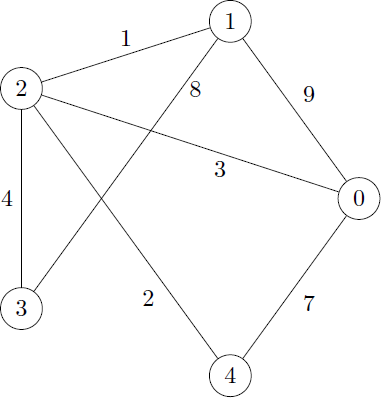
\includegraphics[width=.75\linewidth]{images/exo_3}
\end{center}

\begin{enumerate}
\item Construire la matrice $\left( M_{ij}\right)_{0\leq i,j\leq 4}$, matrice de distances du graphe \texttt{G}, définie par :

<< pour tous les indices $i$, $j$, $M_{ij}$ représente la distance entre les sommets $i$ et $j$,
ou encore la longueur de l’arête reliant les sommets $i$ et $j$ >>.

On convient que, lorsque les sommets ne sont pas reliés, cette distance vaut -1. La distance du
sommet $i$ à lui-même est, bien sûr, égale à 0.
\item Écrire une suite d'instructions permettant de dresser à partir de la matrice \texttt{M} la liste des voisins du sommet 4.
\item Écrire une fonction \texttt{voisins}, d’argument un sommet $i$, renvoyant la liste des voisins du sommet $i$.
\item Écrire une fonction \texttt{degre}, d’argument un sommet $i$, renvoyant le nombre des voisins du sommet $i$, c’est-à-dire le nombre d’arêtes issues de $i$.
\item Écrire une fonction \texttt{longueur}, d’argument une liste \texttt{L} de sommets de \texttt{G}, renvoyant la longueur du trajet d'écrit par cette liste \texttt{L}, c’est-à-dire la somme des longueurs des arêtes empruntées. Si le trajet n’est pas possible, la fonction renverra -1.
\end{enumerate}


\addcontentsline{toc}{subsection}{Exercice 4 -- Gestion de liste}
\subsection*{Exercice 4 -- Gestion de liste}
Soit un entier naturel $n$ non nul et une liste \texttt{t} de longueur $n$ dont les termes valent 0 ou 1. Le but de cet exercice est de trouver le nombre maximal de 0 contigus dans \texttt{t} (c’est-à-dire figurant dans des cases consécutives). Par exemple, le nombre maximal de zéros contigus de la liste \texttt{t1} suivante vaut 4 :
\begin{center}
\begin{tabular}{|c|c|c|c|c|c|c|c|c|}
\hline 
\texttt{i} & 0 & 1 & 2 & 3 & 4 & 5 & 6 & 7 \\
\hline
\texttt{t1[i]} & 0 & 1 & 1 & 1 & 0 & 0 & 0 & 1 \\
\hline
\hline
\texttt{i} & 8 & 9 & 10 & 11 & 12 & 13 & 14 \\
\cline{0-7} 
\texttt{t1[i]} & 0 & 1 & 1 & 0 & 0 & 0 & 0 \\
\cline{0-7}  
\end{tabular}
\end{center}

\begin{enumerate}
\item Écrire une fonction \texttt{nombreZeros(t,i)}, prenant en paramètres une liste \texttt{t}, de longueur n, et un indice i compris entre 0 et $n-1$, et renvoyant :
$$
\left\{
\begin{array}{l}
0, \text{ si } t[i]=1 \\
\text{le  nombre de zéros consécutifs dans t} \\ \text{à partir de t[i] inclus, si t[i] = 0}.
\end{array}
\right.
$$
Par exemple, les appels \texttt{nombreZeros(t1,4)}, \texttt{nombreZeros(t1,1)} et \texttt{nombreZeros(t1,8)} renvoient respectivement les valeurs 3, 0 et 1.
\item Comment obtenir le nombre maximal de zéros contigus d’une liste \texttt{t} connaissant la liste des \texttt{nombreZeros(t,i)} pour $0\leq i \leq n-1$ ?
En déduire une fonction \texttt{nombreZerosMax(t)}, de paramètre \texttt{t}, renvoyant le nombre maximal de 0 contigus d’une liste \texttt{t} non vide. On utilisera la fonction \texttt{nombreZeros}.
\item Quelle est la complexité de la fonction \texttt{nombreZerosMax(t)} construite à la question précédente ?
\item Trouver un moyen simple, toujours en utilisant la fonction \texttt{nombreZeros}, d’obtenir un algorithme plus performant.
\end{enumerate}

\addcontentsline{toc}{subsection}{Exercice 5 -- Probabilités}
\subsection*{Exercice 5 -- Probabilités}
Soient $n$ un entier naturel strictement positif et $p$ un réel compris entre 0 et 1.
On considère $X$ et $Y$ deux variables aléatoires à valeurs dans $\mathbb{N}$ sur un espace probabilisé donné. $X$ suit une
loi de Poisson de paramètre $\lambda = np$ et $Y$ suit une loi binomiale de paramètres $(n, p)$.

\begin{enumerate}
\item Définir une fonction \texttt{Px}, d’arguments $k$, $n$ et $p$, renvoyant la valeur de $P(X = k)$. $k!$ (factorielle k) s’obtient par \texttt{factorial(k)} en Python (bibliothèque math) et \texttt{prod(1 : k)} en Scilab.
Déterminer, pour $n = 30$ et $p = 0,1$, la liste des valeurs de $P(X = k)$ pour $k \in \mathbb{N}$, $0 \leq k \leq 30 $.
\item Définir une fonction \texttt{Py}, d’arguments $k$, $n$ et $p$, renvoyant la valeur de $P(Y = k)$.
On pourra utiliser \texttt{comb} de la sous-bibliothèque \texttt{scipy.misc} en Python et \texttt{binomial} en Scilab.

Déterminer, pour $n = 30$ et $p = 0,1$, la liste des valeurs de $P(Y = k)$ pour $k \in \mathbb{N}$, $0 \leq k \leq 30$.
\item Soit $k \in \mathbb{N}$. On rappelle que, sous certaines conditions sur $n$ et $p$, la probabilité $P(Y = k)$ peut être
approchée par $P(X = k)$. Déterminer une fonction \texttt{Ecart} d’arguments $n$ et $p$, renvoyant le plus grand
des nombres $|P(Y = k) - P(X = k)|$, pour $0 \leq k \leq n$.
\item Soit $e$ un réel strictement positif. Déterminer une fonction \texttt{N}, d’arguments $e$ et $p$, renvoyant le plus
petit entier $n$ tel que \texttt{Ecart(n, p)} soit inférieur ou égal à $e$.
\item Faire l’application numérique dans les quatre cas suivants :
\begin{itemize}
\item $p = 0,075$ avec $e = 0,008$ et $e = 0,005$;
\item $p = 0,1$ avec $e = 0,008$ et $e = 0,005$. Interpréter le dernier résultat.
\end{itemize}
\end{enumerate}


\addcontentsline{toc}{subsection}{Exercice 6 -- Tracer de fonction -- $f(x)=0$}
\subsection*{Exercice 6 -- $f(x)=0$}
On considère la fonction $g$ définie sur $[0 , 2[$ par :
$$ g(x) =
\left\{
\begin{array}{ll}
x &\text{ pour } 0\leq x < 1 \\
1 &\text{ pour } 1\leq x < 2 
\end{array}
\right.
$$
\begin{enumerate}
\item Définir la fonction $g$. Tracer sa courbe représentative sur $[0 , 2[$, c’est-à-dire la ligne brisée reliant les points $(x, g(x))$ pour $x$ variant de 0 à 1,99 avec un pas de 0,01.
\item Définir une fonction $f$ donnée de manière récursive sur $[0 , +\infty[$ par :
$$ f(x) =
\left\{
\begin{array}{ll}
g(x) &\text{ pour } 0\leq x < 2 \\
\sqrt{x} f(x-2) &\text{ pour } x \geq 2
\end{array}
\right.
$$
\item Tracer la courbe représentative de $f$ sur $[0,6]$.
\item Écrire les instructions permettant de calculer, à $10^{-2}$ près, la plus petite valeur $\alpha > 0$ telle que $f(\alpha) > 4$.
\end{enumerate}

\addcontentsline{toc}{subsection}{Exercice 7 -- Algorithmique }
\subsection*{Exercice 7 -- Algorithmique }

On considère le code Python de la fonction \texttt{d} suivante :

\begin{py}
\begin{python}
def d(n):
    L =[1]
    for nombre in range(2,n+1):
        if n%nombre == 0:
            L.append(nombre)
    return L
\end{python}
\end{py}

\begin{enumerate}
\item Quel est le résultat de l’appel \texttt{d(4)} ? Puis de l’appel \texttt{d(10)} ?
Que fait la fonction \texttt{d} ?
\item Un diviseur non-trivial d’un entier \texttt{n} est un diviseur de \texttt{n} différent de 1 et de \texttt{n}. Écrire une fonction \texttt{DNT}, d’argument \texttt{n}, renvoyant la liste des diviseurs non-triviaux de l’entier \texttt{n}.
\item Écrire une fonction \texttt{sommeCarresDNT}, d’argument \texttt{n}, renvoyant la somme des carrés des diviseurs non-triviaux de l’entier \texttt{n}.
\item Écrire la suite des instructions permettant d’afficher tous les nombres entiers inférieurs à 1000 et égaux à la somme des carrés de leurs diviseurs non-triviaux. Que peut-on conjecturer ?
\end{enumerate}

\addcontentsline{toc}{subsection}{Exercice 8 -- Chiffrer -- déchiffrer}
\subsection*{Exercice 8 -- Chiffrer -- déchiffrer}
Soit n un entier vérifiant $n \leq 26$. On souhaite écrire un programme qui code un mot en décalant chaque lettre de l'alphabet de $n$ lettres.
Par exemple pour $n = 3$, le décalage sera le suivant :
\begin{center}
\begin{tabular}{|l|c|c|c|c|c|c|c|c|c|}
\hline
Avant décalage & a & b & c & ... & x & y & z \\
\hline
Après décalage & d & e & f & ... & a & b & c \\
\hline
\end{tabular}
\end{center}
Le mot \texttt{oralensam} devient ainsi \texttt{rudohqvdp}.
\begin{enumerate}
\item Définir une chaîne de caractères contenant toutes les lettres dans l’ordre alphabétique (caractères en
minuscule).
\item Écrire une fonction \texttt{decalage}, d’argument un entier \texttt{n}, renvoyant une chaîne de caractères contenant
toutes les lettres dans l’ordre alphabétique, décalées de \texttt{n}, comme indiqué ci-dessus.
\item Écrire une fonction \texttt{indices}, d’arguments un caractère \texttt{x} et une chaîne de caractères \texttt{phrase}, renvoyant
une liste contenant les indices de \texttt{x} dans \texttt{phrase} si \texttt{x} est une lettre de phrase et une liste vide sinon.
\item Écrire une fonction codage d’arguments un entier \texttt{n} et une chaîne de caractères \texttt{phrase}, renvoyant
\texttt{phrase} codé avec un décalage de \texttt{n} lettres.
\item Comment peut-on décoder un mot codé ?
\end{enumerate}



\addcontentsline{toc}{subsection}{Exercice 9 --  Fractale de Mandelbrot}
\subsection*{Exercice 9 -- Fractale de Mandelbrot}

On pose $M = 20$ et $m = 10$. À un nombre $c$ quelconque, on associe la suite $(u_n)_{n\geq 0}$ définie par $u_0 = 0$ et $u_{n+1} = u_n^2 + c$ pour $n \geq 0$.

S’il existe, on note $k$ le plus petit entier tel que l’on ait $0 \leq k \leq m$ et $|u_k| > M$.
On définit alors la fonction $f$ par 
$$
f : c \mapsto 
\left\{
\begin{array}{l}
k \text{ s'il existe} \\
m+1  \text{ sinon.}
\end{array}
\right.
$$

\begin{enumerate}
\item  Donner le code définissant la fonction $f$.
\item  Tracer l’allure de la courbe représentative de la fonction $f$ sur $[-2; 2]$, en créant une liste \texttt{LX} de 401 valeurs équiréparties entre -2 et 2 inclus et en utilisant les fonctions \texttt{plot} et show de la sous-bibliothèque \texttt{matplotlib.pyplot}.
\item  Construire le tableau des valeurs $f(x+i y)$ où $x$ prend 101 valeurs comprises entre -2 et 0,5 et $y$ prend
101 valeurs entre -1,1 et 1,1. \textit{On rappelle que le nombre complexe $i$ est représenté par $1j$. Par exemple,
le complexe $1 + 2 i$ est représenté par $1+2j$.}
\item  Tracer l’image que code ce tableau. On pourra utiliser les fonctions \texttt{imshow} et \texttt{show} de la sous-
bibliothèque \texttt{matplotlib.pyplot}. Quels paramètres peut-on modifier pour obtenir une meilleure résolution ?
\end{enumerate}


\addcontentsline{toc}{subsection}{Exercice 10 -- Calcul matriciel}
\subsection*{Exercice 10 -- Calcul matriciel}
\textit{Dans cet exercice, avec Python on pourra utiliser la fonction \texttt{array} de la bibliothèque \texttt{numpy}, ainsi que la
fonction \texttt{eig} de la sous-bibliothèque \texttt{numpy.linalg}. Avec Scilab, on utilisera \texttt{spec}.}

\begin{enumerate}
\item Créer deux matrices $R=\begin{pmatrix} 1 & 2 & 3 \\ 4 & 5 & 6  \end{pmatrix}$ et 
$S =\begin{pmatrix} 1 & 2 & 3 \\ 4 & 5 & 6\\ 7 & 8 & 9  \end{pmatrix}$ et les faire afficher.
\item Créer une fonction \texttt{test}, d’argument $M$, renvoyant la valeur \texttt{n} si $M$ est une matrice carrée d’ordre \texttt{n} (entier naturel non nul) et zéro dans tous les autres cas.
Vérifier la fonction test sur $R$ et sur $S$.
\item Le fichier \texttt{ex\_006.txt}, situé dans le sous-répertoire \texttt{data} du répertoire de travail, contient un tableau de valeurs flottantes. Lire ce tableau dans le fichier et vérifier qu’il correspond bien à une matrice carrée d’ordre 5 que l’on désignera par \texttt{M1}. 
\item Déterminer les valeurs propres de la matrice \texttt{M1}.
\item Créer une fonction \texttt{dansIntervalle}, d’arguments une liste $L$ et deux réels $a$ et $b$, renvoyant la valeur \texttt{True} si tous les éléments de la liste $L$ sont dans l’intervalle $[a, b]$ et \texttt{False} sinon. Vérifier que toutes les valeurs propres de la matrice \texttt{M1} sont dans l’intervalle $[0, 1]$.
\end{enumerate}


\addcontentsline{toc}{subsection}{Exercice 11 -- Tri de liste}
\subsection*{Exercice 11 -- Tri de liste}
Soit $N$ un entier naturel non nul. On cherche à trier une liste L d’entiers naturels strictement inférieurs à $N$.
\begin{enumerate}
\item Écrire une fonction comptage, d’arguments $L$ et $N$, renvoyant une liste $P$ dont le $k$-ième élément désigne le nombre d’occurences de l’entier $k$ dans la liste $L$.
\item Utiliser la liste $P$ pour en déduire une fonction \texttt{tri}, d’arguments $L$ et $N$, renvoyant la liste $L$ triée dans l’ordre croissant.
\item Tester la fonction \texttt{tri} sur une liste de 20 entiers inférieurs ou égaux à 5, tirés aléatoirement.
\item Quelle est la complexité temporelle de cet algorithme ? La comparer à la complexité d’un tri par insertion ou d’un tri fusion.
\end{enumerate}

\addcontentsline{toc}{subsection}{Exercice 12 -- Courbes paramétrées}
\subsection*{Exercice 12 -- Courbes paramétrées}
\begin{enumerate}
\item Deux paramètres $b$ et $w$ valant respectivement 0,5 et 6,0, définir trois fonctions d’une variable $t$ renvoyant des couples :
$$
\left\{
\begin{array}{ll}
p : t \mapsto &\left(\cos(t) +b \cos(wt),      \sin(t) + b \sin (wt) \right) \\
v : t \mapsto &\left(-\sin(t)  -bw \sin(wt),\right. \\     
& \quad \left. \cos(t) + b w\cos (wt) \right) \\
a : t \mapsto &\left(-\cos(t)-bw^2 \cos(wt),\right. \\ 
& \quad \left.-\sin(t) - b w^2 \sin (wt) \right) \\
\end{array}
\right.
$$
Vérifier ces fonctions sur un exemple.

$p(t)=(x(t),y(t))$ désigne la position dans le plan d'une masse ponctuelle mobile au cours du temps, $v(t)=(x'(t),y'(t))$, sa vitesse, et $a(t)=(x''(t),y''(t))$, son accélération.
\item Construire la liste \texttt{L} des points $p(t)$, pour $t$ variant de $-\pi$ à $\pi$ avec un pas de discrétisation $\delta t$ vérifiant $\delta t = 0,01 \; \pi$.
\item Faire tracer dans le plan muni d’un repère orthonormal la ligne polygonale reliant les points $p(t)$ de la liste \texttt{L}.
\item Définir puis tester la fonction $c$ d’une variable $t$ qui renvoie le couple des coordonnées du centre de courbure donnée par :
$$
c(t)=\left(x(t)-dy'(t),y(t)+dx'(t)\right) $$ 
où
$$
d= \dfrac{x'(t)^2+y'(t)^2}{x'(t)y''(t)-y'(t)x''(t)}.
$$
\item Rajouter sur le graphique précédent la ligne décrite par les centres de courbure, avec la même
discrétisation en temps.
\item Calculer la longueur de la ligne polygonale reliant les points $p(t)$, pour différents pas de discrétisation $\delta t$. Observer l'évolution de cette longueur lorsque $\delta t$ diminue.
\end{enumerate}


\addcontentsline{toc}{subsection}{Exercice 13 -- Opérations sur les polynômes}
\subsection*{Exercice 13 -- Opérations sur les polynômes -- 2.11.3 p.50}
\begin{flushright}
\textit{D'après Frédéric Butin, l'informatique pas à pas en prépa, éditions ellipses.}
\end{flushright}
Un polynôme $P=\sum\limits_{j=0}^{n}a_j X^j \in \mathbb{R}[X]$ de degré $n$ est représenté dans cet exercice par le tableau $P=[a_0,...,a_n]$.

\begin{enumerate}
\item Créer une fonction \texttt{affiche\_poly} qui permet d'afficher un polynôme sous la forme $P=\sum\limits_{j=0}^{n}a_j X^j$.
\item Créer une fonction \texttt{degre\_poly} qui calcule le degré d'un polynôme.
\item Implémenter la somme, le produit et la multiplication par un scalaire comme des fonctions notées \texttt{add\_poly}, \texttt{mul\_poly} et \texttt{mul\_sca\_poly}.
\item Créer une fonction \texttt{prsc\_poly} qui calcule le prduit scalaire canonique de deux polynômes.
\item Créer une fonction \texttt{deriv\_poly} qui calcule la dérivée d'un polynôme.
\end{enumerate}

\addcontentsline{toc}{subsection}{Exercice 14 -- Produits polynômes}
\subsection*{Exercice 14 -- Produits polynômes -- 2.11.20 p.65}
\begin{flushright}
\textit{D'après Frédéric Butin, l'informatique pas à pas en prépa, éditions ellipses.}
\end{flushright}
Un polynôme $P=\sum\limits_{j=0}^{n}a_j X^j \in \mathbb{R}[X]$ de degré $n$ est représenté dans cet exercice par le tableau $P=[a_0,...,a_n]$.

\begin{enumerate}
\item Créer une fonction \texttt{affiche\_poly} qui permet d'afficher un polynôme sous la forme $P=\sum\limits_{j=0}^{n}a_j X^j$.
\item Créer une fonction \texttt{degre\_poly} qui calcule le degré d'un polynôme.
\item Implémenter le produit de deux polynômes. On notera \texttt{mul\_poly} cette fonction. Donner sa complexité.
\end{enumerate}
On suppose désormais que $n=2^k=2m$. La méthode qui suit permet de calculer le produit de deux polynômes en utilisant le principe <<diviser pour régner>>. 

On pose $P=P_1+X^m P_2$ et $Q=Q_1+X^mQ_2$, où $P_1$ et $Q_1$ sont de degré strictement inférieur à $m$. Ainsi, $PQ=P_1Q_1+X^m\left(P_1Q_2 + Q_1P_2\right)+X^n P_2 Q_2$. 

\begin{enumerate}
\item Calculer le produit de deux polynômes de degré strictement inférieur à $n$ revient donc à calculer 4 produits de deux polynômes de degré inférieur à $\dfrac{n}{2}$. Implémenter cet algorithme en une fonction \texttt{mul\_poly\_div}. Quelle est sa complexité ? Qu'en conclure ?
\item Une autre méthode de calcul consiste à poser $R_1=P_1Q_1$, $R_2=P_2Q_2$ et $R_3=\left(P_1+P_2 \right)\left(Q_1+Q_2 \right)$. Expliciter $PQ$ en fonction des polynômes $R_1$, $R_2$, $R_3$. En déduire un algorithme (appelé algorithme de Karatsuba) permettant le calcul de $PQ$ que l'on implémentera en une fonction \texttt{mul\_poly\_kara}. Comparer la complexité de cet algorithme à celle des algorithmes des questions précédentes. 
\item Que faire quand $n$ n'est pas de la forme $2^k$.
\end{enumerate}


\addcontentsline{toc}{subsection}{Exercice 15 -- Courbes en polaires}
\subsection*{Exercice 15 -- Courbes en polaires -- 4.6.25 p.111}
\begin{flushright}
\textit{D'après Frédéric Butin, l'informatique pas à pas en prépa, éditions ellipses.}
\end{flushright}

Pour tout $n \in \mathbb{N}^*$, on considère $\Gamma_n$ en coordonnées polaires définie par :
$$
\sigma_n(\theta) = \cos^3 \left( n\theta\right) - \sin^3 \left( n\theta\right).
$$
\begin{enumerate}
\item Représenter la courbe $\Gamma_0$.
\item Représenter sur un même graphique les courbes $\Gamma_j$, pour $j \in \llbracket 0,3\rrbracket $.
\end{enumerate}


\addcontentsline{toc}{subsection}{Exercice 16 -- Fonction de Takagi}
\subsection*{Exercice 16 -- Fonction de Takagi -- 4.6.26 p.112}
\begin{flushright}
\textit{D'après Frédéric Butin, l'informatique pas à pas en prépa, éditions ellipses.}
\end{flushright}

La fonction de Takagi est définie sur $[0,1]$ par $T:x\mapsto \sum\limits_{k=0}^{\infty} \dfrac{d\left( 2^k x \right)}{2^k}$, où $d(y)$ représente la distance de $y$ à l'entier le plus proche. On peut montrer que cette fonction est continue sur $[0,1]$ mais nulle part dérivable.
\begin{enumerate}
\item Pour tout entier $n\in \mathbb{N}$, majorer $||T-T_n||_{\infty}=\sup\limits_{x\in[0,1]} |T(x)-T_n(x)|$ où $T_n:x \mapsto \sum\limits_{k=0}^{n} \dfrac{d\left( 2^k x \right)}{2^k}$.
\item Représenter le graphe de cette fonction, appelé la courbe du blanc-manger.
\end{enumerate}

\addcontentsline{toc}{subsection}{Exercice 16 -- Modèle logistique}
\subsection*{Exercice 16 -- Modèle logistique -- 4.6.27 p.113}
\begin{flushright}
\textit{D'après Frédéric Butin, l'informatique pas à pas en prépa, éditions ellipses.}
\end{flushright}

Pour tout $a\in]0,3]$,  on considère la suite récurrente $(u_n)_{n\in\mathbb{N}}$ définie par $u_0 \in \left[ 0,1+\dfrac{1}{a}\right]$ et pour tout $n\in\mathbb{N}^*$, $u_{n+1}=\left(1+a\left(1-u_n \right) \right)u_n$. Cette suite représente, à un facteur près, la population d'une espèce.

\begin{enumerate}
\item Pour $a=1$ et $u_0=0,5$, représenter graphiquement les 10 premiers termes de la suite.
\item On fixe $u_0=0,5$. Créer une procédure qui reçoit en arguments $a_1$, $c$, $a_2$ et permet de représenter les termes $u_n$ pour $n\in \llbracket 100,200 \rrbracket$ et $a=a_1+jc$, $j\in\llbracket 0,\lfloor \dfrac{a_2-a_1}{c}\rfloor \rrbracket$ (les points sont à tracer sont des points de coordonnées $(a,u_n)$.
\item Exécuter cette procédure avec $a_1=2$, $c=0,005$, $a_2=3$ puis avec $a_1=2.84$, $c=0,0001$, $a_2=2,86$.
\end{enumerate}


\addcontentsline{toc}{subsection}{Exercice 17 -- Enveloppe d'une famille de droites}
\subsection*{Exercice 17 -- Enveloppe d'une famille de droites -- 4.6.28 p.115}
\begin{flushright}
\textit{D'après Frédéric Butin, l'informatique pas à pas en prépa, éditions ellipses.}
\end{flushright}

Doit $\left(D_t\right)_{t\in I}$ une famille de droites du plan affine, où $I$ est un intervalle de $\mathbb{R}$. On munit le plan d'un repère, de sorte que la droite $D_t$ a pour équation :
$$
u(t) x+v(t) y + w(t) = 0.
$$

On suppose que les applications $u$, $v$, $w$ sont de classe $\mathcal{C}^1$ sur $I$ et qu'elles ne s'annulent pas en même temps. 

On cherche une courbe paramétrée $f:I \to \mathbb{R}^2$ telle que pour tout $t\in I$, 
\begin{itemize}
\item $f(t)\in D_t$;
\item $D_t$ est tangente à la courbe en $f(t)$.
\end{itemize}
Quand elle existe, cette courbe est appelée l'enveloppe de la famille de droits $\left(D_t\right)_{t\in I}$. 
\begin{enumerate}
\item On note $f(t)=\left(x(t),y(t)\right)$. Montrer que $\left(x(t),y(t)\right)$ est solution du système :
$$
\left\{
\begin{array}{l}
u(t) x(t) + v(t) y(t)= -w(t) \\
u'(t) x(t) + v'(t) y(t)= -w'(t) \\
\end{array}
\right. .
$$
En déduire qu'au voisinage de tout point $t_0 \in I$ tel que :
$$
\left| 
\begin{array}{cc}
u(t_0) & v(t_0) \\
u'(t_0) & v'(t_0)
\end{array}
\right|
\neq 0
$$,
le système précédent a une unique solution, donnée par :
$$
x(t)=\dfrac{\left| 
\begin{array}{cc}
-w(t) & v(t) \\
-w'(t) & v'(t)
\end{array}
\right|
}{\left| 
\begin{array}{cc}
u(t) & v(t) \\
u'(t) & v'(t)
\end{array}
\right|},
y(t)=\dfrac{\left| 
\begin{array}{cc}
u(t) & -w(t) \\
u'(t) & -w'(t)
\end{array}
\right|
}{\left| 
\begin{array}{cc}
u(t) & v(t) \\
u'(t) & v'(t)
\end{array}
\right|}.
$$
\item Déterminer une paramétrisation de l'enveloppe $E$ de la famille des droites $\left(D_t\right)_{t\in \mathbb{R}}$ d'équation :
$$
\sin(t) x - \cos(t) y -\sin^2(t)=0.
$$
\item Représenter, sur un même graphique, $E$ et plusieurs droites $D_t$.
\end{enumerate}




\addcontentsline{toc}{subsection}{Exercice 18 -- Hypocycloïde}
\subsection*{Exercice 18 -- Hypocycloïde -- 4.6.29 p.117}
\begin{flushright}
\textit{D'après Frédéric Butin, l'informatique pas à pas en prépa, éditions ellipses.}
\end{flushright}

Un cercle $ \Gamma\left(\Omega,r\right)$ roule sans glisser à l'intérieur du cercle $C\left(O,R\right)$ (où $R>r$). On note $M=M(\theta)$ un point de $\Gamma$ dont étudie la trajectoire. On note $\theta$ l'angle $\left( \hat{\vect{i},\vect{O\Omega}}\right)$ et $\varphi$ l'angle $\left( \hat{\vect{\Omega I},\vect{\Omega M}}\right)$. Initialement, $\Omega$ est situé sur l'axe horizontal et $M$ est situé en $I_0$.

\begin{center}
\begin{tikzpicture}
\draw(0,0) circle (2);
\draw({1.6*sqrt(2)/2},{1.6*sqrt(2)/2}) circle (.4);
\draw (-2,0) -- (2,0) node [right] {\small $I_0$};
\draw (0,-2) -- (0,2);
\draw (0,0) node [above left] {$O$} -- ({2*sqrt(2)/2},{2*sqrt(2)/2}) node [above] {\small $I$};
\draw [-latex] (0.5,0) arc (0:45:0.5);
\draw (0.5,0.25) node [right] {$\theta$};
\draw({1.6*sqrt(2)/2},{1.6*sqrt(2)/2}) -- ++ ({.4*sqrt(2)/2},{-.4*sqrt(2)/2}) node [below]{\small $M$};
\draw ({1.6*sqrt(2)/2},{1.6*sqrt(2)/2}) node [above] {\small $\Omega$};
\draw [-latex] ({1.8*sqrt(2)/2},{1.8*sqrt(2)/2}) arc (45:-45:0.2);
\draw (1.24,1.15) node [right] {\footnotesize$\varphi$};
\end{tikzpicture}
\end{center}

\begin{enumerate}
\item Montrer que l'affixe de $M$ est donnée par $z(\theta)=\left(R-r\right) \exp\left(i\theta \right) + r \exp\left(i  m \theta \right)$ où $m=1-\dfrac{R}{r}$. Ainsi, $M$ a pour coordonnées :
$$
\left\{
\begin{array}{l}
x(\theta)= \left(R-r\right) \cos \theta +r \cos \left(m \theta \right) \\
y(\theta)= \left(R-r\right) \sin \theta +r \sin \left(m \theta \right) 
\end{array}
\right. .
$$
\item On choisit $R=4$ et $r=\dfrac{R}{4}$. Représenter la trajectoire de $M$. La courbe obtenue est appelée astroïde. 
\item On choisit $R=4$ et $r=\dfrac{R}{p}$ où $p\in \mathbb{N}$. Représenter, pour différentes valeurs de $p$, $\Gamma\left(\Omega,r\right)$ roulant sur $C\left(O,R\right)$, ainsi que la trajectoire de $M$. La courbe obtenue est appelée hypocycloïde à $p$ rebroussements. 
\item Vérifier que ces points sont effectivement des points de rebroussement.
\end{enumerate}

\newpage


\addcontentsline{toc}{subsection}{Exercice 1 -- Arithmétique -- Corrigé}
\subsection*{Exercice 1 -- Arithmétique -- Corrigé}

\begin{corrige}
$\quad$
\begin{python}
# Question 1
n = 1234
q = n//10
r =  n%q

# r contient le nombre d'unités de n
\end{python}
\end{corrige}

\begin{corrige}
$\quad$
\begin{python}
# Question 2
s=0
while n!=0:
    q=n//10
    r = n%10
    #print(r)
    s=s+r**3
    n=q
\end{python}
\end{corrige}

\begin{corrige}
$\quad$
\begin{python}
# Question 3
def somcube(n):
    """
    Entrées :
     * n, int : nombre
    Sortie : 
     * s, int : somme des cubes du chiffre n
    """
    s=0
    while n!=0:
        q=n//10
        r = n%10
        s=s+r**3
        n=q
    return s
\end{python}
\end{corrige}

\begin{corrige}
$\quad$
\begin{python}
# Question 4
res = []
for i in range (10001):
    if i == somcube(i):
        res.append(i)
\end{python}
\end{corrige}

\begin{corrige}
$\quad$
\begin{python}
# Question 5
def somcube2(n):
    """
    Entrées :
     * n, int : nombre
    Sortie : 
     * s, int : somme des cubes du chiffre n
    """
    nombre=str(n)
    s=0
    for chiffre in nombre :
        s = s+int(chiffre)**3
    return s
    
print(somcube2(1234))
\end{python}
\end{corrige}

\vfill

\columnbreak

\addcontentsline{toc}{subsection}{Exercice 2 -- Intégration -- Corrigé}
\subsection*{Exercice 2 -- Intégration -- Corrigé}

\begin{corrige}
$\quad$
\begin{python}
# Question 1
# ==========
# Le répertoire courant est Exercice_02.
# Le sous-répertoire data contient le
# fichier ex_01.txt.

# On ouvre le fichier en lecture)
fid = open("data\ex_01.txt")

# On charge le fichier dans une liste.
# Chaque élément de la liste correspond à 
# chaque ligne sous forme de chaîne de caractère.
file = fid.readlines()
# On ferme le fichier
fid.close()

LX=[]
LY=[]
for ligne in file :
    ligne = ligne.split(';')
    LX.append(float(ligne[0]))
    LY.append(float(ligne[1]))
\end{python}
\end{corrige}

\begin{corrige}
$\quad$
\begin{python}
# Question 2
# ==========
# Ne pas oublier de charger préalablement 
# import matplotlib.pyplot as plt

plt.plot(LX,LY)
plt.show()
\end{python}
\end{corrige}



\begin{corrige}
$\quad$
\begin{python}
# Question 3
# ==========
def trapeze(x,y):
    res = 0 
    for i in range(1,len(LX)):
        res = res+(LX[i]-LX[i-1])*0.5*(LY[i]+LY[i-1])
    return res
print(trapeze(LX,LY))
\end{python}
\end{corrige}

\begin{corrige}
$\quad$
\begin{python}
# Question 4
# ==========
from scipy.integrate import trapz
# Attention à l'ordre des arguments dans 
# la fonction trapz : les_y puis les_x
# Après l'import, help(trapz) permet d'avoir 
# de l'aide sur la fonction.
print(trapz(LY,LX))
\end{python}
\end{corrige}

\newpage

\addcontentsline{toc}{subsection}{Exercice 3 -- Graphe -- Corrigé}
\subsection*{Exercice 3 -- Graphe -- Corrigé}

\begin{corrige}
$\quad$
\begin{python}
# Question 1
# ==========
# Matrices avec des listes
M=[[0,9,3,-1,7],
      [9,0,1,8,-1],
      [3,1,0,4,2],
      [-1,8,4,0,-1],
      [7,-1,2,-1,0]]
\end{python}
\end{corrige}
%\newpage

\begin{corrige}
$\quad$
\begin{python}
# Question 2 & 3
# ==============
def voisins(M,i):
    """
    Entrées : 
      * M(lst) : graphe
      * i : noeud considéré
    Sortie :
      * v(lst) : liste des voisins
    """
    v = []
    # On cherche les voisins sur une ligne 
    # (on pourrait le faire sur une colonne)
    for j in range(len(M[i])):
        if M[i][j]>0:
            v.append(j)
    return v
    
# print(voisins(M,0))
\end{python}
\end{corrige}


\begin{corrige}
$\quad$
\begin{python}
# Question 4
# ==========
def degre(M,i):
    """
    Entrées : 
      * M(lst) : graphe
      * i : noeud considéré
    Sortie :
      * (int) : nomnbre de voisins
    """
    return len(voisins(M,i))
\end{python}
\end{corrige}

\begin{corrige}
$\quad$
\begin{python}
# Question 5
# ==========
def longueur(M,chemin):
    l = 0
    for i in range(len(chemin)-1):
        if M[chemin[i]][chemin[i+1]]<0:
            return -1
        else :
            l=l+M[chemin[i]][chemin[i+1]]
    return l
    
chemin = [1,2,3,1,4]
print(longueur(M,chemin))        
chemin = [0,4,2,1,0]
print(longueur(M,chemin))
\end{python}
\end{corrige}

\vfill

\columnbreak

\subsection*{Exercice 4}
\begin{corrige}
$\quad$
\begin{python}
# Question 1 
# ==========
def nombreZeros(t,i):
    if t[i]==1:
        return 0
    else : 
        res = 1
        j=i+1
        while j<len(t) and t[j]==0:
            res = res+1
            j=j+1
    return res
# t1=[0,1,1,1,0,0,0,1,0,1,1,0,0,0,0]
# print(nombreZeros(t1,4))
# print(nombreZeros(t1,1))
# print(nombreZeros(t1,8))
\end{python}
\end{corrige}

\begin{corrige}
$\quad$
\begin{python}
# Question 2
# ==========
def nombreZerosMax(t):
    max=nombreZeros(t,0)
    for i in range(1,len(t)):
        tmp = nombreZeros(t,i)
        if tmp>max:
            max = tmp
    return max
print(nombreZerosMax(t1))
\end{python}
\end{corrige}

\begin{corrige}
$\quad$
\begin{python}
# Question 3 et 4
# ================
\end{python}
\end{corrige}
\newpage

\addcontentsline{toc}{subsection}{Exercice 5 -- Corrigé}
\subsection*{Exercice 5 -- Corrigé}

\columnbreak 

\addcontentsline{toc}{subsection}{Exercice 6 -- Corrigé}
\subsection*{Exercice 6 -- Corrigé}
\begin{corrige}
$\quad$
\begin{python}
# Import de fonctions
import matplotlib.pyplot as plt
from math import sqrt
# Question 1 
# ==========
def g(x):
    if x>= 0 and x<1 :
        return x
    elif x>1 and x<2 :
        return 1
xx = [0]
t=0
while t<=1.99:
    t=t+0.01
    xx.append(t)
yy = [g(x) for x in xx]
plt.plot(xx,yy)
plt.show()
\end{python}
\end{corrige}

\begin{corrige}
$\quad$
\begin{python}
# Question 2
# ==========
def f(x):
    if x>=0 and x<2 :
        return g(x)
    else : # x>=2
        return sqrt(x)*f(x-2)
\end{python}
\end{corrige}

\begin{corrige}
$\quad$
\begin{python}
# Question 3
# ==========
xxx = [0]
t=0
while t<=6:
    t=t+0.01
    xxx.append(t)
yyy = [f(x) for x in xxx]
plt.plot(xxx,yyy)
plt.show()
\end{python}
\end{corrige}

\begin{corrige}
$\quad$
\begin{python}
# Question 4
# ==========
# On cherche à résoudre f(x)-4 = 0 sur
# l'intervalle [5,6]
def h(x):
    res = f(x)-4
    return res

a = 5.
b = 6.
while (b-a)>0.01:
    m=(a+b)/2
    if h(m)>0:
        b=m
    else :
        a=m
m=(a+b)/2

if h(m)<0:
    m= m+ abs(b-a)
print(m,h(m))
\end{python}
\end{corrige}

\newpage 

\addcontentsline{toc}{subsection}{Exercice 7 -- Corrigé}
\subsection*{Exercice 7 -- Corrigé}

\begin{corrige}
$\quad$
\begin{python}
# Question 1 
# ==========
def d(n):
    """
    Retourne la liste de tous les diviseurs de n.
    Entrée : 
     * n(int) : entier.
    Sortie : 
     * L(lst) : liste des diviseurs de n.
    """
    L =[1]
    for nombre in range(2,n+1):
        if n%nombre == 0:
            L.append(nombre)
    return L
print(d(4),d(10))
\end{python}
\end{corrige}

\begin{corrige}
$\quad$
\begin{python}
# Question 2 
# ==========
def DNT_01(n):
    return d(n)[1:-1]
def DNT_02(n):
    L =[]
    for nombre in range(2,n):
        if n%nombre == 0:
            L.append(nombre)
    return L
print(DNT_01(4),DNT_02(4))
print(DNT_01(10),DNT_02(10))
\end{python}
\end{corrige}


\begin{corrige}
$\quad$
\begin{python}
# Question 3
# ==========
def sommeCarresDNT_01(n):
    L = DNT_01(n)
    res = [x**2 for x in L]
    return sum(res)
def sommeCarresDNT_02(n):
    L = DNT_01(n)
    res = 0
    for x in L:
        res = res + x*x
    return res
def sommeCarresDNT_03(n):
    L = DNT_01(n)
    res = 0
    for i in range(len(L)):
        res = res + L[i]**2
    return res
print(sommeCarresDNT_01(15),sommeCarresDNT_02(15),
    sommeCarresDNT_03(15))
\end{python}
\end{corrige}


\begin{corrige}
$\quad$
\begin{python}
# Question 4
# ==========
from math import sqrt
for i in range(1001):
    if i == sommeCarresDNT_01(i) :
        print(str(i)+"\t"+str(sqrt(i)))
# Conjecture les nombres recherchés sont 
# les carrés des nombres premiers. 
\end{python}
\end{corrige}


\addcontentsline{toc}{subsection}{Exercice 8 -- Corrigé}
\subsection*{Exercice 8 -- Corrigé}
\begin{corrige}
$\quad$
\begin{python}
# Question 1 
# ==========
chaine = "abcdefghijklmnopqrstuvwxyz"
\end{python}
\end{corrige}

\begin{corrige}
$\quad$
\begin{python}
# Question 2
# ==========
def decalage(chaine,n):
    chaine = chaine[n:-1]+chaine[0:n]
    return chaine
print(chaine,decalage(chaine,3))
\end{python}
\end{corrige}

\begin{corrige}
$\quad$
\begin{python}
# Question 3
# ==========
def indices(x,phrase):
    """
    Recherche des indices de x dans phrase
    Entrée : 
     * x(str) : un caractère
     * phrase(str)
    Sortie : 
     * res(lst) : liste des indices de x
    """
    res = []
    for i in range(len(phrase)):
        if phrase[i] == x:
            res.append(i)
    return res

print(indices("a","akjlkjalkjlkjalkjlkja"))
\end{python}
\end{corrige}

\begin{corrige}
$\quad$
\begin{python}
# Question 4
# ==========
def codage(n,phrase):
    ch = "abcdefghijklmnopqrstuvwxyz"
    ch_c = decalage(ch,n)
    print(ch_c)
    phrase_c=""
    for c in phrase :
        i = indices(c,ch)
        i = i[0]
        phrase_c = phrase_c+ch_c[i]
    return phrase_c
print(codage(3,"oralensam"))
\end{python}
\end{corrige}

\begin{corrige}
$\quad$
\begin{python}
# Question 5
# ==========
# Solution 1 : essayer les 26 permutations, 
# jusqu'à trouver une phrase qui est du sens.
# Solution 2 : statistiquement le e est la lettre
# la plus présente dans la langue française. On
# peut donc déterminer la fréquence d'apparition 
# des lettres. # La lettre la plus fréquente 
# peut être assimilée au "e".
# On calcule ainsi le décalage...
\end{python}
\end{corrige}

\newpage


\addcontentsline{toc}{subsection}{Exercice 9 -- Fractale de Mandelbrot -- Corrigé}
\subsection*{Exercice 9 -- Fractale de Mandelbrot -- Corrigé}
\begin{corrige}
$\quad$
\begin{python}
# Question 1 
# ==========
def suite_u(c,n):
    """
    Calcul de la suite u au rang n.
    Entrées : 
     * c(flt) : nombre quelconque
     * n(int)
    Sortie : 
     * res(flt) : valeur de u(n)
    """
    res = 0
    i=0
    while i!=n:
        res = res*res+c
        i=i+1
    return res
\end{python}
\end{corrige}

\begin{corrige}
$\quad$
\begin{python}
def recherche_k(m,M,c):
    """ Recherche de k """
    k=0
    while k<=m:
        if abs(suite_u(c,k))>M:
            return k
        k=k+1
    return -1
\end{python}
\end{corrige}

\begin{corrige}
$\quad$
\begin{python}
def fonction_f(m,M,c):
    """ Fonction """
    k = recherche_k(m,M,c)
    if k>=0:
        return k
    else :
        return m+1
\end{python}
\end{corrige}

\begin{corrige}
$\quad$
\begin{python}
# Question 2
#===========
import matplotlib.pyplot as plt
m,M=10,20
LX = [-2+4*x/400 for x in range(401)]
LF = [fonction_f(m,M,x) for x in LX]
plt.plot(LX,LF,"*")
plt.show()
\end{python}
\end{corrige}
\begin{center}
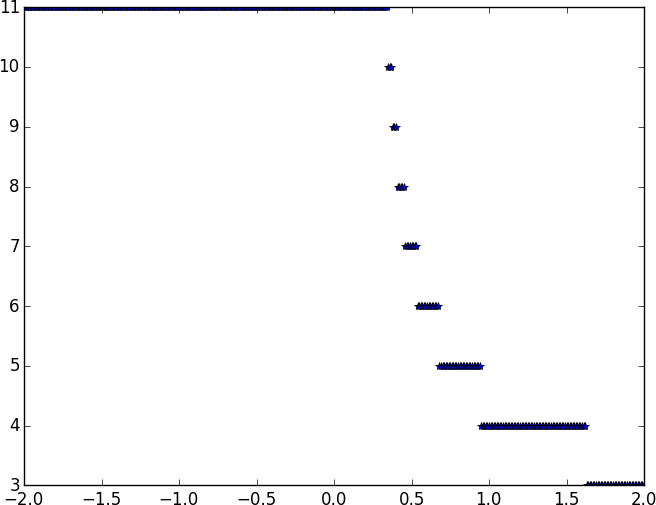
\includegraphics[width=.8\linewidth]{programmes/Exercice_09/figure_1}
\end{center}
\begin{corrige}
$\quad$
\begin{python}
# Question 3
#===========
LX = [-2+2.5*x/100 for x in range(101)]
LY = [-1.1+2.2*x/100 for x in range(101)]
XY = [[[x,y] for x in LX] for y in LY]

for i in range(len(LX)):
    for j in range(len(LY)):
        XY[i][j]=fonction_f(
            m,M,complex(XY[i][j][0],XY[i][j][1]))
\end{python}
\end{corrige}

\begin{corrige}
$\quad$
\begin{python}

# Question 4
#===========
res = 100
LX = [-2+2.5*x/res for x in range(res+1)]
LY = [-1.1+2.2*x/res for x in range(res+1)]
XY = [[[x,y] for x in LX] for y in LY]

for i in range(len(LX)):
    for j in range(len(LY)):
        XY[i][j]=fonction_f(
        m,M,complex(XY[i][j][0],XY[i][j][1]))

# plt.imshow(XY)
# plt.show()
\end{python}
\end{corrige}

\begin{corrige}
$\quad$
\begin{python}

# Bilan 
#=======
def affichage(m,M,res):
    m = m
    M = M
    LX = [-2+2.5*x/res for x in range(res+1)]
    LY = [-1.1+2.2*x/res for x in range(res+1)]
    XY = [[[x,y] for x in LX] for y in LY]
    for i in range(len(LX)):
        for j in range(len(LY)):
            XY[i][j]=fonction_f(
                m,M,complex(XY[i][j][0],XY[i][j][1]))
    plt.imshow(XY)
    plt.show()
\end{python}
\end{corrige}

\begin{center}
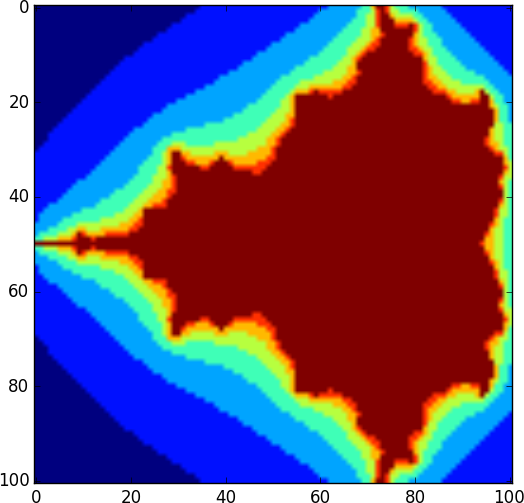
\includegraphics[width=.8\linewidth]{programmes/Exercice_09/10_20_100}

\textit{$m=10$, $M=20$, 100 points par 100 points}
\end{center}

\begin{center}
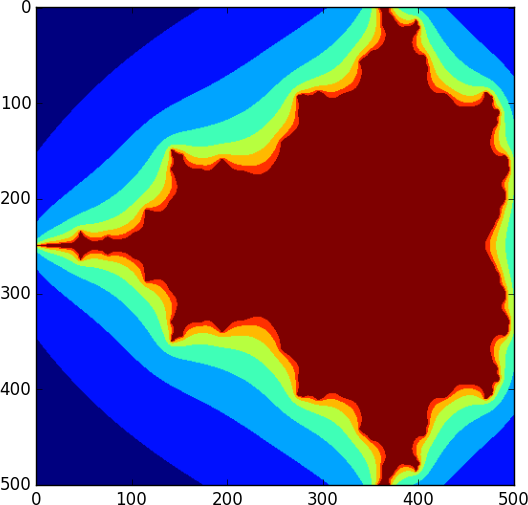
\includegraphics[width=.8\linewidth]{programmes/Exercice_09/10_20_500}

\textit{$m=10$, $M=20$, 500 points par 500 points}
\end{center}

\begin{center}
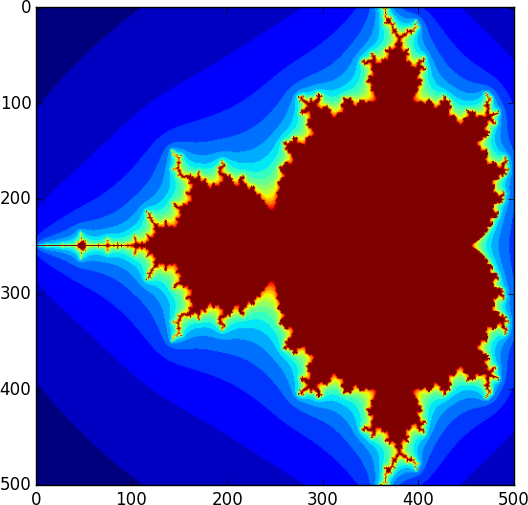
\includegraphics[width=.8\linewidth]{programmes/Exercice_09/20_40_500}

\textit{$m=20$, $M=40$, 500 points par 500 points}
\end{center}

\columnbreak 

\addcontentsline{toc}{subsection}{Exercice 10 -- Corrigé}
\subsection*{Exercice 10 -- Corrigé}
\begin{corrige}
$\quad$
\begin{python}
import numpy as np
# Question 1
R = np.array([[1,2,3],[4,5,6]])
S = np.array([[1,2,3],[4,5,6],[7,8,9]])
\end{python}
\end{corrige}

\begin{corrige}
$\quad$
\begin{python}
# Question 2
def test(M):
    """
    Fonction permettant de tester si la
    matrice est carrée et retournant sa taille.
    Entrée : 
     * M(numpy.ndarray) : matrice
    Sortie :
     * 0 si taille non carrée
     * n(int) : taille de M si elle est carrée
    """
    l = M.shape[0]
    c = M.shape[1]
    if l==c :
        return l
    else : 
        return 0
print(test(R),test(S))
\end{python}
\end{corrige}

\begin{corrige}
$\quad$
\begin{python}
# Question 3
fid = open("data/ex_006.txt",'r')
M1 = []
for ligne in fid :
    l = ligne.rstrip().split(" ")
    Ligne = [float(x) for x in l]
    M1.append(Ligne)
fid.close()
M1 = np.array(M1)
\end{python}
\end{corrige}

\begin{corrige}
$\quad$
\begin{python}
# Question 4
if test(M1)>0:
    valeurs_propres = np.linalg.eig(M1)[0]
    print(valeurs_propres)
\end{python}
\end{corrige}

\begin{corrige}
$\quad$
\begin{python}
# Question 5
def dansIntervalle(L,a,b):
    """
    Vérifier que chaque élément de L est dans 
    l'intervalle [a,b]
    Entrées : 
     * L(lst) : liste de nombres
     * a,b(flt) : nombres
    Sortie : 
     * True si chaque élément est dans [a,b]
     * False sinon. 
    """   
    for e in L :
        if e<a or e> b:
            return False
    return True
print(dansIntervalle(valeurs_propres,0,1))
\end{python}
\end{corrige}

\newpage

\addcontentsline{toc}{subsection}{Exercice 11 -- Tri de liste -- Corrigé}
\subsection*{Exercice 11 -- Tri de liste -- Corrigé}

\begin{corrige}
$\quad$
\begin{python}
# Question 1 
# ==========
def comptage(L,n):
    """
    Comptage des éléments de L.
    Entrées :
     * n(int) : entier
     * L(lst) : liste d'éléments inférieurs à n
    """
    P = [0 for i in range(n+1)]
    # P = [0]*(n+1)
    for e in L:
        P[e]=P[e]+1
    return P
from random import randint
maxi = 5
LL = [randint(0,maxi) for x in range(20)]
P = comptage(LL,maxi)
# print(LL)
# print(P)
\end{python}

\end{corrige}

\begin{corrige}
$\quad$
\begin{python}
# Question 2
# ==========
def tri(L,n):
    """
    Tri une liste.
    Entrées :
     * n(int) : entier
     * L(lst) : liste d'éléments inférieurs à n
    Sortie : 
     * T(lst) : liste triée.
    """
    P = comptage(L,n)
    T = []
    for i in range(len(P)):
        for j in range(P[i]):
            T.append(i)
    return T
\end{python}
\end{corrige}

\begin{corrige}
$\quad$
\begin{python}
# Question 3
# ==========
from random import randint
maxi = 5
LL = [randint(0,maxi) for x in range(20)]
T = tri(LL,maxi)
print(LL)
print(T)
\end{python}
\end{corrige}

\begin{corrige}
$\quad$
\begin{python}
# Question 4
# ==========
# Complexité quadratique : C(n)=O(n+n^2)=O(n^2)
# n : complexité de comptage
# n^2 : complexité des deux boucles imbriquées du 
# tri
# Ce tri s'exécutera toujours dans le pire des cas.
# Dans le cas moyen : tri fusion O(nlogn)
# Dans le cas moyen : tri insertion O(n^2)
\end{python}
\end{corrige}
 
\columnbreak

\addcontentsline{toc}{subsection}{Exercice 12 -- Corrigé}
\subsection*{Exercice 12 -- Corrigé}

\begin{corrige}
$\quad$
\begin{python}
b,w = 0.5,6
# Question 1 
# ==========
import numpy as np
def fonc_p(t):
    return [np.cos(t)+b*np.cos(w*t),np.sin(t)
    			+b*np.sin(w*t)]
\end{python}
\end{corrige}

\begin{corrige}
$\quad$
\begin{python}
def fonc_v(t):
    return [-np.sin(t)-b*w*np.sin(w*t),np.cos(t)
    			+b*w*np.cos(w*t)]
\end{python}
\end{corrige}

\begin{corrige}
$\quad$
\begin{python}
def fonc_a(t):
    return [-np.cos(t)-b*w*w*np.cos(w*t),
    		 -np.sin(t)-b*w*w*np.sin(w*t)]
\end{python}
\end{corrige}

\begin{corrige}
$\quad$
\begin{python}
# Question 2
# ==========
L=np.linspace(-np.pi,np.pi,200)
\end{python}
\end{corrige}

\begin{corrige}
$\quad$
\begin{python}
# Question 3
# ==========
import matplotlib.pyplot as plt
p = fonc_p(L)
#plt.plot(p[0],p[1])
#plt.axis("equal")
#plt.show()
\end{python}
\end{corrige}

\begin{center}
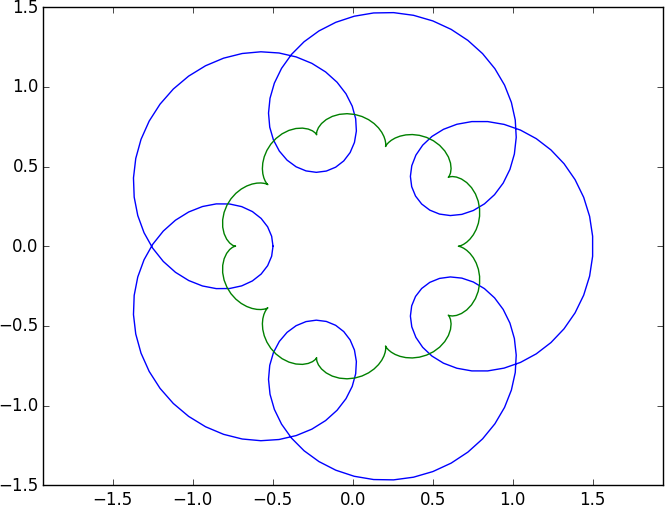
\includegraphics[width=.8\linewidth]{programmes/Exercice_12/figure_1}
\end{center}

\columnbreak

\begin{corrige}
$\quad$
\begin{python}
# Question 4
# ==========
def fonc_d(t):
    xp,yp = fonc_v(t)
    xpp,ypp = fonc_a(t)
    return (xp**2 + yp**2)/(xp*ypp-yp*xpp)
def fonc_c(t):
    fd = fonc_d(t)
    x,y = fonc_p(t)
    xp,yp = fonc_v(t)
    return [x-fd*yp,y+fd*xp]
\end{python}
\end{corrige}

\begin{corrige}
$\quad$
\begin{python}
# Question 5
# ==========
les_xc  = []
les_yc  = []
c = fonc_c(L)
#plt.plot(c[0],c[1])
\end{python}
\end{corrige}

\begin{corrige}
$\quad$
\begin{python}
# Question 6
# ==========
from math import sqrt
def distance(p):
    """
    Calcule la longueur du profil p.
    Entrée : 
     * p(lst) : liste [les_x,les_y]
    Sortie : 
     * L(flt) : longueur du profil.
    """
    L=0
    for i in range(len(p[0])-1):
        x0 = p[0][i]
        y0 = p[1][i]
        x1 = p[0][i+1]
        y1 = p[1][i+1]
        L = L+ sqrt((x1-x0)**2+(y1-y0)**2)
    return L
\end{python}
\end{corrige}

\begin{corrige}
$\quad$
\begin{python}
les_dt = []
les_dist = []
for i in range(10,2000,1) :
    dt = 2*np.pi/i
    L=np.linspace(-np.pi,np.pi,i)
    p = fonc_p(L)
    d = distance(p)
    les_dt.append(dt)
    les_dist.append(d)
plt.plot(les_dt,les_dist)
plt.show()       
\end{python}
\end{corrige}


\begin{center}
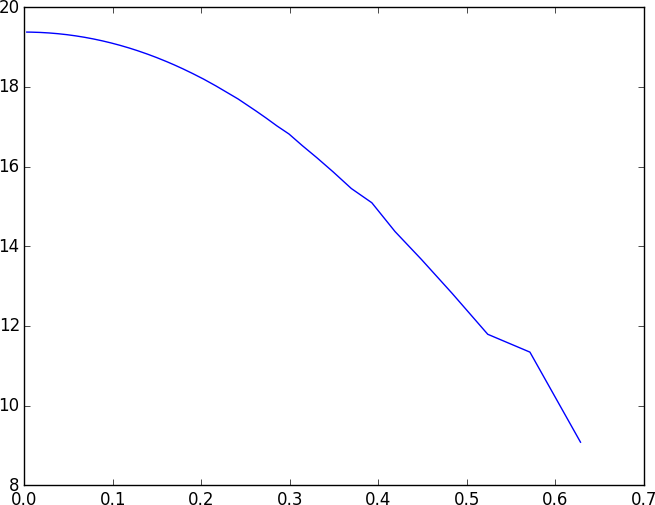
\includegraphics[width=.8\linewidth]{programmes/Exercice_12/figure_2}

\textit{Évolution de la longueur du polynôme en fonction de $\delta t$.}
\end{center}


\end{multicols}
\end{document}







\addcontentsline{toc}{subsection}{Exercice 4}
\subsection*{Exercice 4}

\begin{corrige}
$\quad$
\begin{python}

\end{python}
\end{corrige}

\begin{corrige}
$\quad$
\begin{python}

\end{python}
\end{corrige}

\begin{corrige}
$\quad$
\begin{python}

\end{python}
\end{corrige}

\begin{corrige}
$\quad$
\begin{python}

\end{python}
\end{corrige}

\begin{corrige}
$\quad$
\begin{python}

\end{python}
\end{corrige}




